\documentclass{cisfyp}
\usepackage{apacite}
\usepackage{listings}
\usepackage{multicol}
\usepackage{appendix}

\title{Bioinformatics Resource Portal}
\author{Nigel Alfino}
\supervisor{Mr. Joseph Bonello and Prof. Ernest Cachia}
\date{May \the\year}

\longabstract{Bioinformatics is the field of study that applies computational techniques in order to understand and organise biological data. An obstacle found in performing research in bioinformatics is finding the right tool or dataset to use for that research. This obstacle rises from a lack of effort made in research to make tools or datasets reusable. This issue is also present due to a lack of an indexable resource of tools and datasets, as well as a lack of assessment of their reusability. The FAIR guiding principles provide four principles to measure a tool or dataset's Findability, Accessibiltiy, Interoperability and Reusability, as well as guidelines on how to perform such measurements. This study aims to create a searchable portal of tools, as well as providing an automated assessment tool which provides a FAIR score for tools or datasets based on a set of metrics. This will allow the user to see where the resource struggles to perform and can also refine the score with further information. The FAIR score obtained can provide researchers with a level of trust in the resources they use, as they will be able to properly gauge how Findable, Accessible and Reusable the tool is, and if it can Interoperate with different systems.}

\acknowledgement{I would like to express my deepest gratitude and appreciation to all those who helped and supported me along this journey in completing my dissertation.\newline\newline Firstly, I would like to thank my supervisors, Mr. Joseph Bonello and Prof. Ernest Cachia, for their time and guidance, without which this dissertation would not have been possible.\newline\newline I would also like to thank my friends and family for their constant support, reassurance and encouragement throughout my study. }

\begin{document}

\pagenumbering{roman}
\tableofcontents
\listoffigures
\listoftables
\cleardoublepage
\pagenumbering{arabic}
\setcounter{page}{1}

\chapter{Introduction}
\label{s:intro}

\section{Problem Definition}
In recent years there has been an increase in the number of researchers performing studies in the field of bioinformatics, generating a large amount of tools to solve a wide array of problems in biology \cite{cannata_merelli_altman_2005}. Due to this increase in tools, it has become difficult for researchers to track which tools, datasets and methods are available and useful for their area of study, especially due to the fact that there is no comprehensive index of tools, datasets, and literature annotated with proper metadata \cite{cannata_merelli_altman_2005}.

The increase in the development of tools allowed researchers to be able to process this large amount of data being generated. The ability to process this large amount of data revolutionised research made in the biological field \cite{tools_science}. However, there is limited literature on these tools, which also provides limited information based on the state of the tool when it was created. If updates were made to the tool, changing how a feature works, or increasing the tool's capabilities, these changes are not be covered in the literature \cite{cannata_merelli_altman_2005}. The literature is also not classified by some standard based on the tools' features and capabilities, so finding the right tool can be difficult \cite{cannata_merelli_altman_2005}. Furthermore, the continuous development of tools has led to an increase in this literature, making it even harder for researchers to find the tool they need \cite{grivell_2002}.

In order to ensure the quality of data gathered and used by researchers, a standard must be used to provide a  quality metric for the tools used and research being developed. Research that can be of ``good quality'' can only be achieved through proper data management \cite{Wilkinson2016}. Data must be properly managed in order to produce research of better quality when that data is re-used in new research, either on its own or combined with newly generated data \cite{Wilkinson2016}. The FAIR Guiding Principles \cite{Wilkinson2016} provides four foundational principles that can be used as guidelines by researchers in order to ensure that the data provided in their research is not only properly obtained but also properly managed in order to be reused 
in future research, as well as making it findable to allow for timely generation of data \cite{Wilkinson2016}.
The four principles provided by FAIR are as follows:
\begin{itemize}
	\item Findability
	\item Accessibility
	\item Interoperability
	\item Reusability
\end{itemize}


\section{Approach}
The approach taken in this study involves the implementation of a web application that acts as a searchable repository for bioinformatics tools. A tool will also be developed to automate as much of the assessment of the FAIR score of tools in the repository as possible. The user can then further improve the score by providing any information which the tool might not have been able to find.

The web application will also allow the user to create pipelines of tools, allowing the user to see the FAIR score of the individual tools as well as an overall FAIR score of the pipeline. The user can then identify which tools are 
negatively impacting the FAIR score of the pipeline. 

Evaluation is performed by applying the assessment tool on a set of bioinformatics tools and comparing the FAIR score obtained against the FAIR scores provided for the same tools on FAIRshake \cite{FAIRshake}, which will be used as a benchmark. 

A number of case studies will then be performed using tools which were not evaluated by FAIRshake \cite{FAIRshake}, which will be evaluated using the tool and then manually checked to ensure that the results obtained are as expected.
\pagebreak
\section{Aims and Objectives}
The main aims of this project are as follows:
\begin{itemize}
	\item To conduct an extensive literature review to determine which tools are used in various bioinformatics pipelines;
	\item To build a model to describe the features and capabilities of bioinformatics tools;
	\item To build a tool that automates the assessment of a tool's Findability, Accessibility, Interoperability and Reusability (FAIR) and produces a FAIR score.
\end{itemize}
These aims will be attained through the completion of the following objectives:
\begin{itemize}
	\item To obtain a comprehensive overview of tasks in bioinformatics and which tools are commonly used in the task;
	\item To obtain a searchable archive of tools that can be filtered by task, feature and capability;
	\item To enhance the archive with a FAIR score indicating the Findability, Accessibility, Interoperability and Reusability of the tool to aid researchers make decisions on which tools to use.
\end{itemize}

\section{Research Questions}
This study is aimed to answer the following list of research questions:
\begin{itemize}
	\item Can the features of bioinformatics tools be modelled in such a way to provide a researcher insights into the tool's capabilities and usage context?
	\item Are the tools used in bioinformatics findable through simple searches and can a search provide insights into the tool's capabilities?
	\item Can a FAIR score for a particular tool help the user in finding the appropriate tool for their particular task?
	\item Can the FAIR assessment be part of an automated process?
\end{itemize}
From the above research questions, the following hypothesis was formed:\newline
``Using a centralized repository of bioinformatics tools that captures the important features and capabilities of the tools, and by enhancing this information with a FAIR assessment score, users can make better judgements on which tools are appropriate for a particular bioinformatics pipeline.''


\section{Report Layout}
This first chapter of the report provides a basic explanation on what the study will be addressing, what aims and objectives it aims to achieve as well as provides a brief explanation on how these aims and objectives will be achieved. The rest of the report is organised in the following manner. The second chapter provides information on the background and literature review on the area. The third chapter provides an analysis on how the application was designed. The fourth chapter provides a detailed description of how the application was implemented. The testing and evaluation of results obtained from the application are presented in the fifth chapter. This is followed by future works and finally the conclusions drawn.
\pagebreak

\chapter{Background and Literature Review}
\section{Bioinformatics}
Bioinformatics is a field that consists of multiple disciplines, namely those of computer science, mathematics, statistics, genetics and molecular biology. It is described as applying computational techniques - obtained from applied mathematics, computer science and statistics - in order to understand information and organise it \cite{luscombe2001}. As a research discipline, bioinformatics is viewed as biology involving computation \cite{2011}. Bioinformatics is the field of study that aims to solve, though the use of a computational approach, large scale biological problems that are considered data intensive \cite{yousef_allmer_2014}. Yousef \& Allmer (2014) show how a solution in bioinformatics usually follows the procedure listed below: 
\begin{itemize}
	\item Biological data is collected from statistics.
	\item A computational model is built.
	\item A computational modelling problem is solved.
	\item The computational algorithm is tested and evaluated.
\end{itemize}
Due to the phenomenal rate at which data in biology is being produced, the use of bioinformatics is crucial for researchers to be able to process these large amounts of data, thanks to computers' abilities to process such data with relative ease \cite{luscombe2001}.

The term bioinformatics was first used as early as 1977 by Paulien Hogeweg, a Dutch theoretical biologist, however the term gained a true meaning during the ``Bioinformatics in the 90s'' conference \cite{Attwood2011}. Researchers' need to access and analyse biological data which was being generated at an increasing rate allowed the field of bioinformatics to grow organically. This need, alongside the development of algorithms and resources that allow for analysis and manipulation of large amounts of data allowed the field of bioinformatics to flourish and gain importance within the community of biological research \cite{Attwood2011}.

\subsection{Aims of Bioinformatics}
Research in the field of bioinformatics is made to achieve three main aims: \cite{luscombe2001}
\begin{itemize}
	\item The simplest aim of bioinformatics is to organise data in a manner that would allow researchers to access and manipulate existing data with ease, as well as publish and access data as they are produced.
	\item Research in bioinformatics is focused on developing tools and resources that aid in the analysis of the data gathered. Although the gathering of data is a crucial task, this data is practically useless until it is analysed.
	The development of such tools requires proficiency in computational theory as well as in-depth knowledge in the field of biology. 
	\item The tools developed are used to analyse and interpret the data generated in a biologically meaningful manner. Traditional biological studies analysed systems individually in great detail, however bioinformatics allows ``global analyses with the aim of 
	uncovering common principles that apply across many systems and highlight novel features'' \cite{luscombe2001}.
\end{itemize}

\subsection{Datasets and Tools}
The introduction of computers was the key to handling the data that was being generated \cite{Attwood2011}. Advancements made in computation allowed for the creation of multiple databases and datasets to facilitate the storage and manipulation of this 
large amount of data. These advancements gave rise to the creation of the most popular databases used in bioinformatics today, namely:
\begin{itemize}
	\item NCBI Entrez \cite{Maglott2004}
	\item EBI Ensemble \cite{Flicek2012}
	\item UCSC Genome Browser \cite{Kent2002}
	\item Kegg \cite{Kanehisa2011}
\end{itemize}

Despite great strides made in computation, analysis of biological data still faces many challenges such as noise or incompleteness \cite{yousef_allmer_2014}. Inconsistencies can also arise from data stored on different databases; as well as redundancy in large amounts of overlapping data, not only due to the data being stored in multiple databases, but also due to similar data and datasets used to perform research \cite{yousef_allmer_2014, zvelebil_baum_2008}. Situations have arisen in past research where multiple datasets would need to be combined, each of them containing large amounts of overlapping data. The resulting dataset would end up being too large, making it inefficient to query, thus invalidating the first fundamental aim of bioinformatics \cite{zvelebil_baum_2008}.

On top of all this, each database has its own format on how data is stored and managed \cite{yousef_allmer_2014}. Although research has been carried out in order to maintain a standard such as that of the Gene Ontology consortium \cite{Ashburner2000}, until such a standard is employed throughout the multiple databases, researchers will still have to learn the specifics of each database in order to use it efficiently and effectively \cite{zvelebil_baum_2008}.

\subsection{Pipelines}
The development of tools in the field of bioinformatics has allowed researchers to make great leaps in their discoveries due to the tools' ability process large amounts of data in a timely fashion \cite{tools_science}. However, certain analyses in bioinformatics research that are of a high-throughput nature require the data being analysed to be transformed multiple times, through multiple tools in order to obtain the required result \cite{Leipzig2016}. This series of transformations is called a pipeline \cite{Leipzig2016}. Figure 2.1 shows the basic structure of a pipeline. As can be seen in the figure, a pipeline runs most of its analyses in parallel, as well as involving multiple downstream steps combined with report generation \cite{Leipzig2016}.
\begin{figure}
	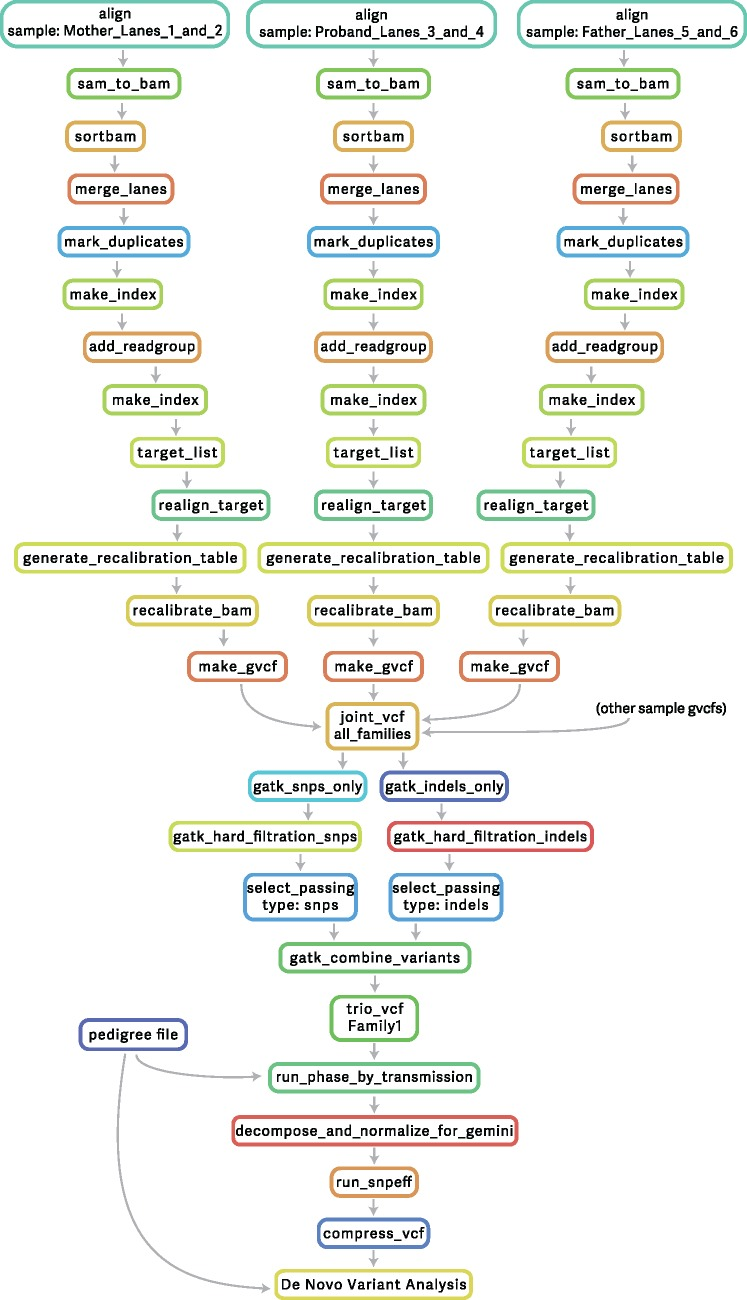
\includegraphics[width=13.5cm, height=22.9cm]{pipeline.jpg}
	\caption{A directed acyclic graph depicting a trio analysis pipeline for detecting de novo mutations, reproduced from Leipzig (2016).}
	\label{fig:pipeline}
\end{figure}\pagebreak

Bioinformatics pipelines consist of both parallel and serial steps, using varied software and data types as well as consisting complex dependencies, with both fixed and user-defined variables and parameters \cite{Leipzig2016}. Modern pipeline frameworks also support more advanced qualities, such as the ability to display the progress of the pipeline in real time, as well as creating environments to run the tool anywhere and providing support for work to be performed on distributed clusters or using cloud technologies \cite{Leipzig2016}.

\section{FAIR Guiding Principles}
Data in bioinformatics is being generated at a very fast rate; however this doesn't mean that we are gaining an increasing amount of knowledge along with this data \cite{Wittig2017}. The main problem stems from the fact that there has been a failure in the storage and organization of this rapidly accumulating data, which should have been stored in ``rigorous, principled ways,'' \cite{Attwood2009} so that the required data can be found easily. This failure has led to exhausting, frustrating, stressful and also expensive experiences when trying to obtain the required data \cite{Attwood2009}.

Furthermore, there is a lack of effort made in scientific research to make results reproducible \cite{nature}. In scientific research, one of the fundamental principles is the independent verification of data. Researchers should be able to re-create experiments and arrive at the same conclusions, thus validating and strengthening the original work whilst allowing for further research based on those results \cite{nature}. However, often times scientific findings cannot be reproduced leading to a waste of time and resources \cite{nature}. This lack of reproducibility makes it difficult to reuse that data which, in turn, lowers the output of scientific research and slows down scientific progress \cite{nature}.

The FAIR principles are guidelines that ensure that data can be found and used by machines, in turn supporting data reuse by individuals. This way, more research of better quality can be generated by ensuring that data, algorithms and the tools and workflows that led to these data were designed to be findable, accessible, interoperable and reusable \cite{2016}.

The goal that we would like to reach is the ease of data integration and reuse by the community after it is published. In order to achieve this goal it is important that data is managed properly \cite{Wilkinson2016}. Publishers, governmental agencies and funders have started requesting researchers to present ``data management and stewardship plans'' \cite{Wilkinson2016}. These plans are required to ensure that the assets provided by the research is properly managed and given long-term care - allowing it to be reused with ease in future research, either by itself or in conjunction with newly generated data. Good data management and stewardship will then ensure high quality digital publications which will in turn further simplify future research \cite{Wilkinson2016}. 

It is difficult, however to properly define what good data management is made up of, as there is no proper standard to ensure data is managed properly. As such, the FAIR guiding principles provide the research community with four foundational principles to improve data management and data stewardship that will in turn increase the value gained by digital publishing: \cite{Wilkinson2016}
\begin{itemize}
	\item Findability.
	\item Accessibility.
	\item Interoperability.
	\item Reusability.
\end{itemize}

These principles act as guidelines, and conditions for data sharing, encouraging researchers to ensure that the data being generated can be shared and reused from the outset \cite{Boeckhout2018}. The FAIR principles highlight the importance of metadata and metadata standards with regards to data stewardship. Metadata  is the ``information and attributes applying to datasets and the data contained therein'' \cite{Boeckhout2018}. These principles stress the need that metadata and metadata standards should be articulated and made readily and publicly available - allowing for further Reusability and reproducibility of data in the scientific field \cite{Boeckhout2018}.

Furthermore, these guidelines ensure that the metadata can be indexed, retrievable and analysed through the use of computers. Automation in data retrieval is important in research made on large-scale programs that use large amounts of data because it allows researchers to obtain data in an easier, more efficient manner. The FAIR principles also ensure that the terms and conditions under which the data can be shared and accessed are ``explicit, well-defined and readily available'' \cite{Boeckhout2018}. This includes any constraints in gaining or granting access to the data, privacy of the data, and publication rights. Although calls have been made in favour of open data, the FAIR principles instead offer  a middle-ground - ``the aim is to settle on legitimate and effective means of controlling access while facilitating bona fide research for all data''  \cite{Boeckhout2018}.

The FAIR principles aim to achieve a step toward ``machine-actionability - where a digital object provides detailed information to an autonomously-acting, computational data explorer'' \cite{Wilkinson2016}. This would allow for the data to be obtained in a timely manner, as computers can retrieve data at a much faster rate than humans, while also maintaining some of the semantic importance that is given by humans in the process of searching for data \cite{Wilkinson2016}.

It is important to note that these principles do not only apply to formal digital publishing and its data, but also to the tools, pipelines and algorithms that led to the creation of this data. The application of these principles to all aspects of research and data generation will be beneficial to all forms of digital research, whether it is data or analytical pipelines, since their availability can ensure transparency, Reusability and reproducibility \cite{Wilkinson2016}.

The FAIR guiding principles benefit a number of stakeholders by ensuring the Reusability of data, mainly researchers who can obtain and publish data in a timely manner, but also publishers, software developers who provide processing services and funding agencies \cite{Wilkinson2016}. However, these stakeholders have differing interests in the effect of FAIR, therefore any metrics that arise from these guidelines need to provide benefits for all the different stakeholders' interests \cite{Wilkinson2018}.

Wilkinson et al. state that a good metric should have the following properties: \cite{Wilkinson2018}
\begin{itemize}
	\item Clear: the purpose of the metric can be easily understood by anyone;
	\item Realistic: the metric should not be complicated for a resource to abide by;
	\item Discriminating: the metric should measure something that impacts FAIRness; evaluate to what degree that resource has achieved that metric; and provides instruction on how this value can be maximized;
	\item Measurable: the assessment of the metric can be made in an ``objective, quantitative, machine-interpretable, scalable and reproducible manner, ensuring transparency of what is being measured and how.;''
	\item Universal: the metric must be applicable to all digital resources
\end{itemize}

If the aims of FAIR were to be realised and implemented, the end result would be more rigorous data management and data stewardship of digital resources, which would provide a benefit to the entire academic community \cite{Wilkinson2016}. To this end, a
set of guidelines were created to aid researchers to create digital research artefacts that are more findable, accessible, interoperable and reusable. Although these guidelines and principles are not a standard or specification, they are a step forward in order to ensure FAIRness of data.

In order to fully understand the aims presented by FAIR, it is important to first understand what is truly meant by findability, accessibility, interoperability and reusability, as well as understanding these guidelines that ensure FAIRness of data.\pagebreak



\subsection{Findability}
Findability is the first principle in FAIR. The guidelines presented by the principle of findability focuses on the requirement that the data being generated is made findable - i.e. The data is easy to find. This is a crucial prerequisite to the other three principles presented by FAIR \cite{Wise2019}.

Wilkinson et al. (2016) describe findability as - ``data should be identified using globally unique, resolvable and persistent identifiers, and should include machine-actionable contextual information that can be indexed to support human and machine discovery of that data.''

To this end, the following set of guidelines were formally given to ensure findability of data: 
\begin{itemize}
	\item Data is properly described using rich metadata;\item Data and metadata are assigned a globally unique identifier;\item Metadata clearly and explicitly includes an identifier of the data it describes;\item Data and metadata are registered and/or indexed in a public searchable resource;\item Data, metadata and their identifiers should be re-findable at any point in time, thus should be persistent;\item Data should contain some basic machine actionable metadata which separates and distinguishes it from other data objects.
\end{itemize}

Findability of data can then be further enhanced by ensuring the use of standard identifiers and annotations, as well as through the use of standard ontologies and databases \cite{Wittig2017}. Further enhancement can be made through the use of a controlled vocabulary. This will ensure that information is unambiguous - use of identifiers based on standards ensures that certain abbreviations have only one meaning and ensures that there will be no variation in the schemas of metadata \cite{Wittig2017, Wise2019}. The result would be the production of models that might use different terminologies but can be used simultaneously, which will further build on the aim of ensuring findability of data.
The key performance indicators that ensure findability of data include sufficient metadata that will allow users and machines to understand the data, additional documentation as well as the availability of uniform resource identifiers (URIs) or persistent identifiers (PIDs) \cite{Wise2019}.


\subsection{Accessibility}
The second principle in FAIR is that of accessibility. Accessibility addresses the necessity to make newly generated and previously existing data as well as digital assets more accessible \cite{Wise2019}. Accessibility ensures that metadata and data are understandable to both humans and machines as well as ensuring that the data is stored in a trusted repository \cite{libereurope_2017}.
Accessibility is based on three main components: \cite{Wise2019}
\begin{itemize}
	\item Access protocol - i.e. Information is provided on how to access the data; \item Access authorisation - i.e. Information is provided on what authorisation (if any) is required to access the data; \item Metadata longevity - i.e. Ensuring that the metadata provided will remain accessible, even if the data itself is not.
\end{itemize}
Usually, the data generated through research has a defined and finite lifespan, however, the metadata that corresponds with that data should ideally be stored permanently, so that the scientific record of the original data would be permanently stored \cite{Wise2019}. It is also important that the protocols used for access authorisation are made public, making it easy to determine who is authorised to gain access of the data \cite{Wise2019}.

It should be noted that data does not need to be made open to be FAIR. Accessibility dictates only the access and authorisation protocols be clearly defined and use open standards. Privacy requirements can still be observed \cite{Wise2019}.

To ensure accessibility of data, the following set of guidelines were formally presented: \cite{Wilkinson2016}
\begin{itemize}
	\item Data and metadata are retrievable by their identifier using a standardised communications protocol;
	\item The communications protocol used to retrieve data and metadata is open, free and universally implementable;
	\item The communications protocol allows for authentication and authorisation procedures, where necessary;
	\item The metadata related to the data remains accessible, even after the data becomes unavailable;
	\item Both humans and machines must be able to judge the actual accessibility of each data object.
\end{itemize}


\subsection{Interoperability}
The third principle in FAIR is that of interoperability. The principle of interoperability ensures that data being used can be integrated with other data, as well as being able to interoperate with other applications and workflows used for analysis, storage and processing of data. To ensure interoperability, the metadata should use a formal, accessible, shared and broadly applicable language for knowledge representation \cite{libereurope_2017}.

The strategies used to achieve interoperability are essentially linked with the other FAIR principles. According to FAIR, data and metadata must be expressed in a formal, accessible, shareable and broadly applicable language \cite{Wise2019}. As such, observing standards when generating data will automatically drive data integration at all levels \cite{Wise2019}.

To achieve interoperability, the following guidelines were formally provided: \cite{Wilkinson2016}
\begin{itemize}
	\item Data and metadata use a formal, accessible, shared and broadly applicable language for knowledge representation;
	\item Data and metadata use vocabularies that follow FAIR principles;
	\item Data and metadata include qualified references to other data and other metadata;
	\item Data and metadata are machine-actionable;
	\item Data and metadata formats use shared ontologies;
	\item Data and metadata within the data object are both syntactically parseable as well as semantically machine-accessible.
\end{itemize}

The Interoperability of generated data can be further improved through the use of common exchange formats \cite{Wittig2017}. A widely-used example of such a format in systems biology is SBML - Systems Biology Markup Language \cite{Hucka2003}. Such formats would allow for the automatic and machine-readable exchange of data and facilitate the development of automatic data workflows between data management systems, applications and databases \cite{Wittig2017}.\pagebreak

\subsection{Reusability}
The final principle in FAIR is that of Reusability. The optimisation of reuse of data is the ultimate goal of FAIR. It is what separates traditional data management from FAIR data stewardship \cite{Wise2019}. Reusability ensures that data and collections have clear usage licenses and provide accurate information on provenance \cite{libereurope_2017}.

Reusability is mainly achieved through well described data and metadata, allowing them to be replicated and combined in different settings \cite{gofair}.

It allows for the re-purposing of data for new needs, applications and user communities \cite{Wise2019}. Reusability allows data to ``become more valuable to more people across large organisations, whether open-source communities or private organisations'' \cite{Wise2019}.

To achieve this ultimate goal of Reusability, the following guidelines were formally presented: \cite{Wilkinson2016}
\begin{itemize}
	\item Data objects should be compliant with the first three principles of FAIR - i.e They must be findable, accessible and interoperable;
	\item Data and metadata are richly described with a plurality of accurate and relevant attributes;
	\item Data and metadata are released with a clear and accessible data usage license;
	\item Data and metadata are associated with detailed provenance;
	\item Data and metadata meet domain-relevant community standards;
	\item Data and metadata should be sufficiently described and rich enough that it can be linked, integrated automatically or with minimal human effort;
	\item Published data objects should refer to their sources with rich enough metadata and provenance to enable proper citation.
\end{itemize}

The reusability of data is further enhanced by providing proper descriptive information about its context. This includes any information about the original source where the data was obtained, as well as information about the procedures of how the data was generated. Further information about unique data attributes further enhances the reusability \cite{Wittig2017}. This enhanced reusability allows researchers to fully understand the algorithms, data used and the context with regards to an experiment as well as to fully understand the conclusions drawn from the study \cite{taylor2008}.

\section{Conclusion}
In this chapter, research made on bioinformatics, the datasets and tools used in bioinformatics was reviewed in order to understand the background of the area that this study is being performed. The literature review documented the problems regarding the ever increasing amount of data being generated in the field of biology, as well as the organisation and management issues that arise from them from a bioinformatics standpoint.

It also reviews the aims in the FAIR principles, as well as the\newline guidelines presented along with these principles in order to assure FAIRness of data. It can be noted that some of the advantages presented by the use of these guidelines would allow researchers to overcome the problems found in the processing of data in bioinformatics. 

As such, this study focuses on finding a way to automate as much as possible a system that provides a FAIR score for tools and datasets, providing researchers a means to gauge the findability, accessibility, interoperability and reusability of their research. 
\pagebreak
\chapter{Specification and Design}
\section{Overview}
The main goal for this study is to create a tool that semi-automates the FAIR assessment of bioinformatics tools and datasets, while allowing users to refine the score through a portal. The portal can also be used to allow the user to search for a particular tool or dataset, view that particular tool or dataset's performance in terms of a FAIR score as well as create pipelines of tools and datasets, automatically calculating the pipeline's FAIR score based on the tools and datasets used. 

The metrics that will be used to calculate a FAIR score for tools were obtained from the FAIRshake tool rubric \cite{FAIRshake}. Some adjustments and further enhancements, were made to these metrics to be better suited for the tool's performance. Additional metrics were also added in order to ensure a more accurate FAIR score.

The metrics that will be used to calculate the FAIR score for datasets were obtained from the following sources:
\begin{itemize}
	\item The FAIRshake dataset rubric \cite{FAIRshake};
	\item  The Australian Research Data Commons (ARDC) FAIR self-assessment tool \cite{ands}.
\end{itemize}

The sets of tools and datasets that will be used to evaluate the system are split as follows:
\begin{itemize}
	\item Tools from the FAIRshake tool rubric assessments \cite{FAIRshake} will be used to evaluate and match the results obtained by the tool using FAIRshake as a benchmark;
	\item Datasets from the FAIRshake dataset rubric assessments \cite{FAIRshake} will be used to evaluate and match the results of the tool using FAIRshake as a benchmark;
	\item Tools and datasets that will be used as case studies obtained from the European Bioinformatics Institute services \cite{ebi};
	\item Pipeline as presented by \cite{Barber2012} will be used as an additional case study.
\end{itemize}
\section{FAIR Guidelines}
The principles presented by FAIR are meant to be applied generally to all facets of research and data generation. This of course includes ensuring FAIRness of software artefacts. However, since the guidelines presented by \cite{Wilkinson2016} \textit{Guiding Principles for Findable, Accessible, Interoperable and Re-usable Data Publishing version b1.0}, 2016, are meant to be broad so that they can be applied to different fields as needed, they cannot be used as metrics to calculate a FAIR score in their proposed form \cite{dbcls}.

The main focus of this study is to create a tool that semi-automates the FAIR assessment of tools and datasets. Therefore, these guidelines need to be further expanded to create metrics that can be used to properly assess software and datasets respectively. 

As such, in order to find out how the FAIR principles can be properly applied to software the following set of questions must first be answered \cite{dbcls}:
\begin{itemize}
	\item Which FAIR principles can be directly adopted?
	\item Which FAIR principles can be adapted for software, and how?
	\item Are there any guidelines that do not apply to software, and can thus be dismissed?
	\item What should be added to the principles in order for them to apply for software?
\end{itemize}
\pagebreak
\subsection{Findability Guidelines}
In order to apply the guidelines provided by FAIR to ensure findability in software and datasets, certain adjustments might need to be made to them. Furthermore certain guidelines need to be further defined to be applied for software \cite{dbcls}.

Taking a look at the guidelines presented by FAIR to ensure findability, the following changes and further definitions can be made for the guidelines to account for software artefacts and datasets \cite{dbcls}:
\begin{itemize}
	\item \textbf{Data is assigned a globally unique and persistent identifier.}\newline
	This is one of the guidelines presented by the principle of findability. When applied to certain types of data, such as research papers or books, this can refer to a DOI or an ISBN. However, software does not contain this type of public identifier.
	
	Tools in bioinformatics, however, are always presented along with a research paper describing the tool's capabilities, features, tests and experiments performed with it. This paper contains its own unique and persistent DOI. As such, for the purpose of this study, the DOI of the paper which presented the tool will be used as its identifier.
	\item \textbf{Data is described with rich metadata.}\newline
	The tool needs to be described properly in terms of its features and capabilities. Although these will be listed and explained in the paper that presents the tool, it is important that they can be easily found by the user.
	\item \textbf{Data is registered or indexed in a searchable resource.}\newline
	By uploading datasets, tools and their metadata to a website, this requirement can be fulfilled through the use of a search engine. This will allow them to be found easily by searching for certain terms that can match either the dataset or tool's name or a tool's capabilities. 
	
	By storing the metadata on the website, a researcher would also be fulfilling the previous requirement. 
	
	Furthermore, only by fulfilling this guideline can the assessment of the tool's accessibility, interoperability and reusability be performed. This guideline ensures that the tool is findable in the most trivial sense. If the tool is not findable at all, then it's accessibility, interoperability and reusability cannot be assessed.
\end{itemize}\pagebreak

\subsection{Accessibility Guidelines}
Similar to the guidelines to ensure findability, the guidelines presented for the principle of accessibility also needed to be changed or defined further in order to be applied for software.

The following changes were made to ensure that the guidelines for accessibility can account for software and datasets: \cite{dbcls}
\begin{itemize}
	\item \textbf{Metadata and data are retrievable by their identifier using a standardised communications protocol.}\newline
	Both metadata and data should be retrievable in some manner. Given that the DOI, the metadata of the tool or dataset, in this case represented by the research paper, should be retrievable via HTTP or HTTPS. Furthermore, since the tool or dataset will be hosted on a website, this website should also be accessible and retrievable via HTTP and HTTPS.
	
	\item \textbf{The metadata related to the data remains accessible, even after the data becomes unavailable.}\newline
	This guideline ties in with one of the guidelines presented for findability. It is important that the DOI of the research paper presenting the tool or dataset is findable due to the fact that, if for some reason, the website containing the data is down, there will be no access for the metadata related to the tool.
	
	Furthermore, the DOI allows a tool's metadata to be preserved in the case that, for some reason, the tool becomes outdated and as such is no longer supported. 
	
	\item \textbf{Information should be provided on how a tool can be accessed.}\newline
	This is the most important aspect of ensuring the accessibility of a tool. Since the guidelines themselves are intended to be generic so that they can be applied to different aspects of research, there is no specific guideline on how to handle accessibility of software. As such, this is a proposed added guideline to aid in the assessment of software to ensure the generation a proper FAIR score. 
	
	Through this guideline, the metadata related to the tool should be enhanced slightly to include information that would not be included otherwise in other types of data, as for such types it would be irrelevant. The metadata should include with it information on how to access the tool, whether it is through API usage or a sequence of operations performed through a command line interface. 
	
\end{itemize}\pagebreak

\subsection{Interoperability Guidelines}
The guidelines presented by FAIR to ensure interoperability are mainly focused on ensuring that metadata is properly understandable and shareable. However some of these guidelines are not applicable with regards to tools and datasets. 

As such some of these guidelines must be further defined, as well as adding an additional guideline as can be seen below \cite{dbcls}:
\begin{itemize}
	\item \textbf{Metadata and data use a formal, accessible, shared and broadly applicable language for knowledge representation.}\newline
	The metadata related to the tool or dataset must be expressed in a way that can be properly understood and properly follow rules of some knowledge representation language. This applies to the data of a dataset itself. However, in the case of tools, the data refers to the source code of the tool, which cannot be assessed by such a guideline. An argument can be made, however, that following proper coding practices and obeying syntactic and semantic rules of programming languages used can server as an equivalent for a knowledge representation language. \cite{dbcls}
	
	\item \textbf{Data and metadata use vocabularies that follow FAIR principles}\newline
	This guideline states that the chosen language used to represent the metadata and data within the datasets should be openly accessible and follow FAIR principles. In the case of software, since the data is the source code of the tool, this guideline does not apply.
	
	\item \textbf{Data and metadata include qualified references to other data or metadata.}\newline
	As a minimum requirement to fulfil this guideline, the software should use well-known vocabularies to express what inputs and what outputs are accepted.
	
	Furthermore, proper referencing must be made with regards to what other tools or research was used in order to create the tool or dataset.
\end{itemize}

As can be seen above, the guidelines to ensure interoperability are not applicable when the data to be assessed is a software artefact. As such, the following guideline is proposed so that the interoperability of software can be properly assessed:
\begin{itemize}
	\item \textbf{Metadata must properly indicate how the data, in this case the software, interacts with the system it is being used on.}\newline
	This guideline states that software metadata can be further defined to also include how the software interacts with the system it is being executed on. This includes information on compatibility with different operating systems, as well as availability of source code.
\end{itemize}\pagebreak
\subsection{Reusability Guidelines}
Given that reusability is the ultimate goal of FAIR, it is important to ensure that the guidelines presented by this principle are further defined to be applicable for software.

As such, the following definitions were provided to ensure that software's reusability can be properly assessed \cite{dbcls}:
\begin{itemize}
	\item \textbf{Data and metadata are richly described with multiple accurate and relevant attributes.}\newline
	Similar to the guidelines presented by findability, ensuring that the tools and datasets are properly described through their metadata will ensure that the data can be findable through their metadata. Furthermore, being provided with the proper metadata will ensure that the tools and datasets can be re-used in the future, as it will allow the user to understand them and how to use them. 
	
	\item \textbf{Data and Metadata are released with a clear and accessible data usage license.}\newline
	It is important to make sure that the license of the metadata is properly understood. Furthermore you must make sure that you have a license for your software.
	
	The license for both the data and metadata must both be properly presented so that the evaluator can properly assess the tool.
	
	\item \textbf{Data and metadata are associated with detailed provenance.}\newline
	Information on when the software was first created, along with the first experiments and tests that were executed on it should be made available. Furthermore, although the metadata - which will be preserved in the research paper - should not change, if amendments are made to the paper, the original paper should still be made available along with the amendments.
\end{itemize}
Although these guidelines cover some aspects of a software's reusability, in order to ensure that the software's reusability is properly assessed, the following guideline is proposed:
\begin{itemize}
	\item \textbf{Data and metadata are available in a public resource.}\newline
	This guideline, similar to the guideline provided by the principle of findability, states that the data and metadata can both be found publicly. With the metadata being made available in a public resource, the information is available for when the software is to be re-used. Moreover, if the data is stored in a public repository, it will automatically ensure that the data can be found and be 
	made readily available for re-use.
\end{itemize}
\section{FAIR Metrics - Tools}
After further defining the FAIR guidelines to ensure that they can be applied to software, the metrics that will be used within our system to evaluate the FAIR score of bioinformatics tools will be defined. Most of these metrics are based on research previously made by FAIRshake (2018) with a few more metrics being proposed to ensure the generation of a more accurate FAIR score.

\subsection{Tool Findability Metrics}
For the purpose of this study, the metrics provided by the FAIRshake (2018) tool rubric proved to be enough to cover the findability score of a tool, along with an additional metric to better adhere to the adjusted guidelines as proposed by \cite{dbcls}.

Furthermore, certain metrics were given a higher priority to ensure that tools that are wholly findable get a better score to properly represent their better Findability when compared to other tools.\newline
The metrics used in the system to assess findability are as follows:
\begin{itemize}
	\item \textbf{Tool is findable on a website.}\newline
	This is a metric that must be satisfied. If a website is not found for the bioinformatics tool, the FAIR assessment tool will not be able to automate the assessment. Satisfying this metric ensures that the tool adheres to the guideline, i.e., data is registered in a publicly searchable resource \cite{Wilkinson2016}.
	
	\item \textbf{Tool is freely downloadable.}\newline
	This metric is given a high priority, since if a tool is freely downloadable, its findability is greatly increased. 
	
	\item \textbf{A proper description is provided for the tool.}\newline
	This metric is given a medium priority. Satisfying this metric ensures that the tool adheres to the guideline, i.e., data is described by rich metadata \cite{Wilkinson2016}.
	
	\item \textbf{Previous versions of the tool are made available.}\newline
	This metric is given a low priority. Satisfying this metric ensures that the tool adheres to the guideline, i.e., data should be re-findable at any point in time and thus should be persistent \cite{Wilkinson2016}.
	
	\item \textbf{Tool has a unique identifier.}\newline
	This metric is given a medium priority. This metric states that the tool must have a unique identifier, in this case a DOI linked to the paper that presented the tool. Satisfying this metric ensures that the tool adheres to the guideline, i.e., data is assigned a globally unique identifier \cite{Wilkinson2016}.
	
\end{itemize}

\subsection{Tool Accessibility Metrics}
The metrics provided by the FAIRshake (2018) tool rubric do not cover much in terms of accessibility, providing only one metric which needed to be adjusted slightly in order to be automated. Together with this metric another metric is proposed to ensure a proper assessment of the tool's accessibility.\newline
The metrics used in the system to assess accessibility are as follows:
\begin{itemize}
	\item \textbf{Tool can be programmatically accessed through an API.}\newline
	This metric is given a medium priority. Satisfying this metric ensures that the tool adheres to the proposed guideline, i.e., information should be provided on how the tool can be accessed.
	
	\item \textbf{Tool can be accessed through a set of commands executed in a command line interface.}\newline
	This metric is given a high priority. Satisfying this metric also ensures that the tool adheres to the proposed guideline. However, it is given a higher priority as if it can be accessed through a command line interface then it can be accessed by any system.
\end{itemize}

\subsection{Tool Interoperability Metrics}
The FAIRshake (2018) tool rubric does not provide any metrics for interoperability. As such, in order to be able to assess the interoperability of the tools, the following two metrics are proposed:
\begin{itemize}
	\item \textbf{Tool compatibility information is provided.}\newline
	This metric is given medium priority. This metric states that proper information is provided on which operating systems this tool is compatible with. Satisfying this metric ensures that the tool adheres to the proposed guideline. Metadata must properly indicate how the tool interacts with different operating systems. The 
	assessment of this tool is split into 3 parts:
	\begin{itemize}
		\item Windows compatibility,
		\item Linux compatibility, and
		\item Mac compatibility.
	\end{itemize}
	\item \textbf{Tool source code is provided.}\newline
	This metric is given medium priority. This metric assumes that if a tool's source code is provided then it can be executed provided that the system it is executed on has a source-compatible compiler for the programming language in which the tool was written. Satisfying this metric ensures that the tool adheres to the proposed guideline that metadata must properly indicate how the tool interacts with different operating systems.
\end{itemize}
\subsection{Tool Reusability Metrics}
For the purpose of this study, the metrics provided the by the FAIRshake (2018) tool rubric prove to be enough to provide a proper assessment of a tool's reusability score. As such, the same metrics were adopted to be used for the system.\newline
The metrics used in the system to assess reusability are as follows:
\begin{itemize}
	\item \textbf{Tool is hosted in a public repository.}\newline
	This metric is given a high priority. This metric states that the tool must be hosted on a public repository such as GitHub. Satisfying this metric ensures that the tool adheres to the proposed guideline that data is available in a public resource.
	
	\item \textbf{Tool uses community accepted ontologies.}\newline
	This metric is given medium priority. This metric states that if the tool uses one or more ontologies, these ontologies must be stated and must adhere to some standard. If the tool does not use an ontology, this metric will not apply and as such will not affect its FAIR score. Satisfying this metric ensures that the tool adheres to the guideline, i.e., data and metadata meet domain-relevant community standards \cite{Wilkinson2016}.
	
	\item \textbf{Proper documentation of the tool is provided.}\newline
	This metric is given medium priority. This metric states that proper documentation on how to use the tool must be provided. Satisfying this metric ensures that the tool adheres to the guideline, i.e., data and metadata are richly described with a plurality of accurate and relevant attributes \cite{Wilkinson2016}.
	
	\item \textbf{Developer contact information is provided.}\newline
	This metric is given low priority. This metric increases the tool's reusability in such a way that if an issue arises during use of the tool, one can easily contact the developer with their issues in order to have them resolved.
	
	\item \textbf{Information on how to cite the tool is provided.}\newline
	This metric is given low priority. Satisfying this metric ensures that the tool adheres to the guideline, i.e., published data objects should refer to their sources with rich enough metadata and provenance to enable proper citation \cite{Wilkinson2016}.
\end{itemize}

\section{FAIR Metrics - Datasets}
The aim of this study is to create a tool that automates the FAIR assessment for tools and datasets. After defining the metrics that will be used to assess the FAIR score of tools, the metrics that will be used to assess datasets can be defined. Most of these metrics are adopted directly from, or based on the research previously made by FAIRshake (2018) and the nectar-rds FAIR Assessment Tool (2018).

\subsection{Dataset Findability Metrics}
For the purpose of this study, the metrics provided by the FAIRshake (2018) dataset rubric prove to be enough to provide a proper assessment of a dataset's findability score. As such, the same metrics were adopted to be used for the system.\newline
The metrics used in the system assess findability are as follows:
\begin{itemize}
	\item \textbf{Dataset is findable on a website.}\newline
	Similar to the metric used to find tools, this is the most important metric as if the dataset fails it, the FAIR assessment tool will not be able to automate the assessment.
	
	\item \textbf{Dataset has a proper description.}\newline
	This metric is given medium priority. Satisfying this metric ensures that the dataset adheres to the guideline, i.e., data is described by rich metadata \cite{Wilkinson2016}.
	
	\item \textbf{Dataset has a unique identifier.}\newline
	This metric is given low priority. This metric states that the dataset must have a unique identifier, in this case a DOI linked to the paper that originally presented the dataset. Satisfying this metric ensures that the dataset adheres to the guideline, i.e., data is assigned a globally unique identifier \cite{Wilkinson2016}.
\end{itemize}
\pagebreak
\subsection{Dataset Accessibility Metrics}
For the purpose of this study, metrics were adapted from both the FAIRshake (2018) dataset rubric, as well as from the nectar-rds FAIR Assessment Tool (2018).\newline
The metrics used in the system to assess accessibility are as follows:
\begin{itemize}
	\item \textbf{Dataset is freely downloadable from the website.}\newline
	This metric is given a high priority. If the dataset can be freely downloaded, its accessibility is improved greatly.
	
	\item \textbf{Metadata will still be available even if data is no longer available.}\newline
	This metric is given a low priority. Assuming that the dataset has a unique identifer linking it to the paper that originally presented the dataset, then this metric is automatically satisfied.\newline
	Satisfying this metric ensures that the dataset adheres to the guideline, i.e., the metadata related to the data remains accessible, even after the data becomes unavailable \cite{Wilkinson2016}.
\end{itemize}
\subsection{Dataset Interoperability Metrics}
The FAIRshake (2018) dataset rubric does not provide any metrics for the analysis of interoperability of datasets. The nectar-rds FAIR Assessment Tool (2018) provides one metric which can be directly adopted into the system.\newline
As such, the metric used in the system to assess interoperability is as follows:
\begin{itemize}
	\item \textbf{Information is provided on which format(s) or file format(s) the dataset is available in.}\newline
	This metric is given medium priority. In the case of datasets, interoperability is improved when the dataset comes in formats that can be used in conjunction with multiple varying tools and datasets. As such, having the information on which formats the dataset is available in will greatly improve the dataset's interoperability.\newline
	Satisfying this metric ensures that the dataset adheres to the guideline, i.e., data and metadata use a formal, accessible, shared and broadly applicable language for knowledge representation \cite{Wilkinson2016}.
\end{itemize}
\subsection{Dataset Reusability Metrics}
For the purpose of this study, the metrics provided by the FAIRshake (2018) dataset rubric are be enough to provide a proper assessment of a dataset's reusability. As such, the same metrics were adopted for the system.\newline\newline
The metrics used in the system to assess the reusability are as follows:
\begin{itemize}
	\item \textbf{Information is provided on how to cite the dataset.}\newline
	This metric is given low priority. Satisfying this metric ensures that the tool adheres to the guideline, i.e., published data objects should refer to their sources with rich enough metadata and provenance to enable proper citation \cite{Wilkinson2016}.
	
	\item \textbf{Contact information is provided for the creator(s) of the dataset.}\newline
	This metric is given low priority. The ability to contact the creator or creators of the dataset in case something is unclear or some further information is need improves the reusability of the dataset.
	
	\item \textbf{Previous versions of the dataset are made available.}\newline
	This metric is given a low priority. Satisfying this metric ensures that the dataset adheres to the guideline, i.e., data should be re-findable at any point in time and thus should be persistent \cite{Wilkinson2016}.
\end{itemize}

\section{Gathering of Data}
The main function of the system is that given a name of a dataset or a tool, search the web for information about the tool or dataset and try to gather as much information from the metadata found in order to generate a FAIR score for that tool or dataset. This search can be further narrowed down if the URL itself is given. Furthermore, the system should be able to calculate the FAIR score of a pipeline that is defined by the user.
In order to be able to test such a function, multiple sets of data were gathered to ensure that the evaluation of the system was done to verify and validate the system's capabilities.

To evaluate the system, the sets of data needed to include sets of tools and datasets to evaluate the system's ability to generate FAIR scores. The set of tools consists of:
\begin{itemize}
	\item Tools obtained from the FAIRshake (2018) tool rubric assessment.\newline
	This is a set of tools on which assessment was performed by the FAIRshake (2018) tool. This assessment will serve as a benchmark against which the system's score will be compared. Although some of the metrics may be different and there may be some new metrics involved, the system should be able to provide a similar FAIR score to that of the assessment made by the FAIRshake (2018) tool.
	
	\item Tools obtained from the EMBL-EBI tool service \cite{ebi}.\newline
	The EMBL-EBI is a service that hosts some of the most commonly used tools \cite{ebi}. Given that these tools are popular and used often, it is expected that these tools should generate a favourable FAIR score. Some of the tools will be assessed by the system, and then a manual assessment will also be performed on them. These will serve as case studies to ensure that the tool performs as expected.
	
	\item Datasets obtained from the FAIRshake (2018) dataset rubric assessment.\newline
	Similar to the set of tools that was obtained from the tool rubric assessment, this is a set of datasets on which an assessment was performed using the FAIRshake (2018) dataset rubric. The assessment will serve as a benchmark against which the system's score will be compared. Similarly, although some of the metrics may be different, the system is expected to provide 
	a similar FAIR score to that of the assessment made by the FAIRshake (2018) dataset rubric assessment.
	
	\item Datasets obtained from the EMBL-EBI dataset service \cite{ebi}.\newline
	The EMBL-EBI also hosts some commonly used datasets \cite{ebi}. An assumption is made where given that the hosted datasets are popular and used quite often, these datasets should perform well when assessed by the system, generating a favourable FAIR score. Therefore, a small set of these datasets will 
	be assessed by the system, and then be manually assessed. Similarly to the tools, these will serve as case studies to ensure that the tool performs as expected.
\end{itemize}
An extra set of data must be collected in the FAIR assessment of tools. As stated in one of the metrics used to assess a tool's Reusability, a tool must use community accepted ontologies. A list of community accepted ontologies has been compiled. For the purpose of this study, this list of ontologies is compiled from the OBO Foundry. The OBO Foundry provides a table 
of used ontologies and their status, whether they are active, inactive or obsolete \cite{obo}. For the purpose of this study, the list of active ontologies will be used as the set of community accepted ontologies.

Finally, the system's capability to generate a FAIR score for a pipeline that will be built by the user must be evaluated. In order to evaluate this function, a sample pipeline was obtained from research performed by \cite{Barber2012}. The tools and datasets in the pipeline presented by \cite{Barber2012} will be passed through the system, having a FAIR score generated, which will then be double-checked by performing a manual assessment. A FAIR score for the pipeline will then be calculated from the FAIR scores of these tools and datasets. \newline\newline

\begin{figure}[h]
	\centering
	\includegraphics[width=13.5cm]{untitled.jpg}
	\caption{A visual representation of the pipeline presented by Barber et al. (2012), reproduced from \textit{Conflicting Evolutionary Patterns Due to Mitochondrial Introgression and Multilocus Phylogeography of the Patagonian Freshwater Crab Aegla neuquensis} (2015)}
	\label{fig:pipeline}
\end{figure}\pagebreak
\chapter{Implementation}
\section{System Architecture}
This chapter will discuss the computation involved in the implementation of the system, as well as the technologies used to implement it. In this section, a basic overview of the system architecture will be given.

The system is built using Python and its main supporting library Django (2018), a web framework for Python. This allowed for the creation of the FAIR assessment tool and back-end processing of the portal using Python and other supporting libraries. The portal was then built using the various functions provided by Django to design the views and templates while using an HTML front-end.

The FAIR assessment tool was built using web crawling techniques provided by the Selenium package for Python to obtain information about the tools and datasets from online sources, along with additional Python logic to calculate scores for findability, accessibility, interoperability and reusability. The scores obtained from the FAIR assessment tool are then stored in a MySQL database. This database holds the FAIR scores of the various tools and datasets in the system along with some additional information about them. When the user checks for further information about the tool, along with which areas need information to be able to obtain a better FAIR score, summary information about the tool is provided, such as the tool's description, where to download the tool and the DOI of the paper where the tool was presented.

The portal itself acts as a front-end for the user to be able to see what tools and datasets are in the system and their FAIR scores. The user can then see the full details on a tool or dataset, allowing them to find out what can be added to or changed in the tool or dataset's website in order to increase that tool or dataset's FAIR score. The user can then manually refine the score by providing any information which the automated assessment tool might have missed. An example of this relates to the second metric provided by this study for reusability: a tool must use a community accepted ontology. This metric would need to be refined manually, as there is no way for the automated tool to tell whether a tool uses an ontology or not. As such, it is automatically assumed that the tool uses one, but it was not listed. The user is then told that if the tool uses an ontology, listing which ontologies are used would increase its reusability, but if it does not use an ontology, then the user can refine the score by marking the metric as not applicable to the tool. Once the user finishes adjusting the information, the FAIR score is re-calculated in the back end. 

The following sections will discuss what technologies were used, how the FAIR assessment tool was implemented and the additional data to aid in calculating the FAIR assessment was obtained.
\section{Technologies Used}
In this section the main technologies used in the study along with the supporting libraries that were used in order to implement the solution will be discussed.
\subsection{Development Software}
The system was written in Python 3.7 (2018). A portal was then created using Django 2.1 (2018) which is a web framework for Python 3.7 (2018). Thanks to Python's ability to quickly integrate systems together, the FAIR assessment tool was then integrated into the portal.

The IDE used to develop the system was Visual Studio Code (2015). A MySQL database was used which was hosted on an Apache (2018) server started through XAMPP (2017). This allowed for the use of phpMyAdmin 4.8.2 (2018) to manage the database.
\subsection{Supporting Libraries}
In order to implement the system, this study made use of some freely available Python libraries to allow for rapid development. To install these libraries, pip was used, which is a package-management system used to install and manage software packages written in python. \pagebreak

\begin{table}[h]
\resizebox{\textwidth}{!}{%
{\renewcommand{\arraystretch}{1.5}%
\begin{tabular}{|c|l|}
\hline
\textbf{Django 2.1 (2018)} & \begin{tabular}[c]{@{}l@{}}High-level Python Web framework. Provides necessary\\ tools for web development that were used to develop the Portal.\end{tabular} \\ \hline
\textbf{mysqlclient (2018)} & Library that allows Python to interact with a MySQL database. \\ \hline
\textbf{\begin{tabular}[c]{@{}c@{}}Google API \\ Python Client (2018)\end{tabular}} & \begin{tabular}[c]{@{}l@{}}Provides the necessary tools to allow Python to interact with tools \\ provided by Google API. Used to implement website search through \\ Google Custom Search (2006).\end{tabular} \\ \hline
\textbf{Selenium Python (2018)} & \begin{tabular}[c]{@{}l@{}}Provides the necessary tools to perform web crawling using Python. \\ To use this library, the proper driver had to be downloaded to allow \\ Selenium to interface with the browser. In the study the application \\ interacts with Firefox. As such, the driver that had to be installed was \\ geckodriver (2018).\end{tabular} \\ \hline
\textbf{PyYAML (2018)} & \begin{tabular}[c]{@{}l@{}}Library that allows Python to parse YAML files. Used to parse the list \\ of active ontologies obtained from the OBO foundry (Smith et al., 2007), \\ which was obtained in a YAML format.\end{tabular} \\ \hline
\textbf{\begin{tabular}[c]{@{}c@{}}Crossref API Python \\ Client (2018)\end{tabular}} & \begin{tabular}[c]{@{}l@{}}Provides functions that allow Python to iterate through the Crossref API. \\ \\ Used in order to obtain DOI of papers that presented the tools and datasets.\end{tabular} \\ \hline
\end{tabular}%
}}
\caption{List of supporting libraries.}
\label{tab:my-table}
\end{table}

\section{FAIR Assessment Tool}
In this section the implementation of the assessment tool will be discussed. The process begins by having the user input the name of the tool or dataset to be assessed. Using the Google Custom Search API, a list of links is found using the name of the tool or dataset as a search phrase. For the purpose of this study, this list is limited to a maximum of 20 links. These links are then filtered to attempt to find the official website for the tool or dataset to begin crawling for information. This is done by comparing the data found in the website with a list of terms that are related to and commonly used in bioinformatics listed in listing 4.1.
\begin{lstlisting}[frame = single, caption={List of most commonly used phrases in bioinformatics.}, captionpos=b]
phrases = ["protein", "dna", "bioinformatics", "genome", 
	"nucleotide", "biological", "biotechnology", 
	"alignment", "amino acid", "autoradiography", 
	"autosomal", "blotting", "blots", "cell", 
	"computational biology", "sequencing", 
	"similarity", "cluster", "cytoplasm", "enzyme",
	"gene", "genomics", "immunoglobuline", 
	"lead", "mitosis"]
\end{lstlisting}
Once a website is found, the link will be used by Selenium to obtain information and perform the assessment. A slight drawback in the implementation of the system is that a website can be found that would not be the official website of the tool or dataset, however it would contain one or more phrases from the list of phrases most commonly used in bioinformatics and would be used to try and obtain information. The information gathered would not be relevant to the tool or dataset on which the assessment would be performed, resulting in an incorrect assessment.

Given this drawback, Selenium proves to be the perfect tool to obtain information in order to perform the assessment. Although there are more efficient tools for web crawling, Selenium allows you to see which websites the program is accessing and which links it is following. This ensures that the website being crawled is the correct one.
When integrated with the portal, the user is given the option to also provide the link for the tool's official website, further ensuring that the assessment is performed correctly.
\subsection{Tool FAIR Assessment}
This section will consider the computation involved in performing a FAIR assessment for a tool. This starts by considering the most important metric presented in this study for Findability, i.e., the tool is findable on a website. If no website is found after filtering the links found from the Google Custom Search API, then the assessment will automatically fail, as there is no way to gather information to automate the assessment.\newline
\begin{figure}
\centering
\begin{minipage}{.5\textwidth}
  \centering
  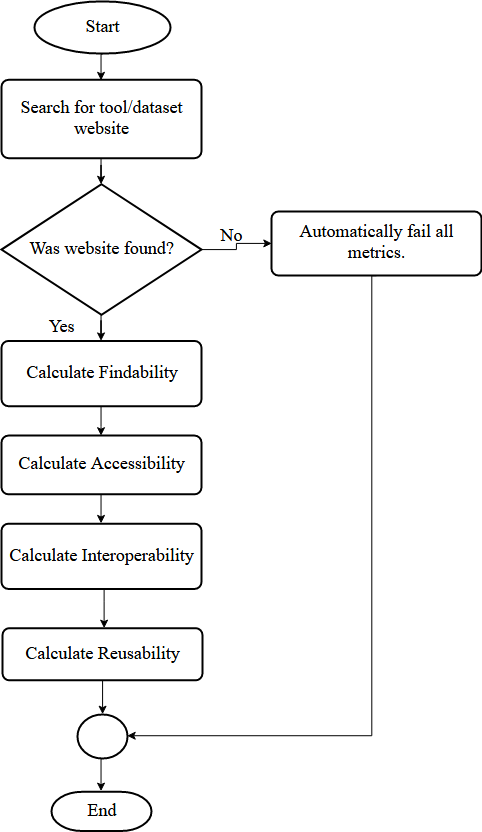
\includegraphics[width=.85\linewidth]{Flowchart1.png}
  \captionof{figure}{Flowchart showing start of FAIR assessment.}
  \label{fig:test1}
\end{minipage}\qquad
\begin{minipage}{.4\textwidth}
  \centering
  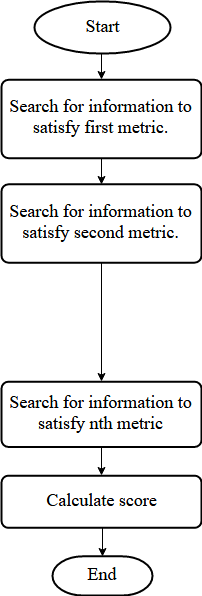
\includegraphics[width=.6\linewidth]{Flowchart2.png}
  \captionof{figure}{Sample flowchart of an assessment.}
  \label{fig:test2}
\end{minipage}
\end{figure}

\textbf{Findability}\newline
The assessment tool then goes on to search for information based on the second metric, that the tool is freely downloadable. This is implemented by first checking if the website is hosted on a GitHub repository, in which case it is automatically assumed that the tool is freely downloadable and marked as such. Otherwise, the website is searched for a link marked ``Download''. If such a link is found, then the score is given, otherwise it is given a zero score. This metric was given a high priority equal to 40\% of the total findability score.

The tool then searches for information for the third metric, i.e., a proper description is provided for the tool. This is implemented by first searching for a link that would redirect the tool to a page providing information about the tool. If no such link is found, the tool then searches for areas on the page marked either as ``Introduction'', ``About'' or ``Description''. If no such area is found, the tool then searches by XPath to see if an area in the HTML would be marked as ``desc''. If the information required is found, the description of the tool is saved into the database and the score for this metric is given. This metric was given a medium priority, equal to 25\% of the total findability score.

The assessment tool then searches for information based on the fourth metric presented by the study, i.e., previous versions of the tool are made available. This is implemented by searching the page for links or areas labelled as either ``Older versions'' or ``Previous versions''. If such an area is found then the tool is given points for this metric. If the driver is in a GitHub link, however, it is assumed that previous versions can be accessed within the repository, therefore a full score would be awarded. This metric carries 10\% of the total findability score, as it was given a low priority.

The assessment tool then goes on to search for information based on the final metric presented in this study, that the tool has a unique identifier. This is implemented by first searching the page for a link containing a DOI, which could be used as a direct link to the paper that presented that tool. If such a link is not found, the tool interfaces with Crossref using the Crossref API to search for the paper that presented the tool by searching for the tool's name. If a paper is found, the DOI is directly extracted from the paper and saved into the database, awarding points to the tool for the metric. This metric was given a medium priority and a score of 25\% of the total findability score is assigned.
\begin{lstlisting}[frame = single, caption={Extracting DOI from paper.}, captionpos=b]
tool_doi = item[`DOI']
\end{lstlisting}
\textbf{Accessibility}\newline
After calculating the tool's findability, the assessment tool starts crawling the website for information to calculate its accessibility. It first begins by searching for information to cover whether the tool can be programmatically accessed through an API. This is done by first searching for a link marked with the text ``API'', which would link you to a page providing information on how to access the tool from an API. If such a link is not found, the page is instead checked for areas marked with the text ``API''. If such a link is found then the score for this metric is awarded. Since this metric is marked as medium priority, it carries 50\% of the total accessibility score.

The assessment tool then searches for information based on the second metric, i.e., the tool can be accessed through a set of commands executed in a command line interface. This is implemented by searching through the web page for areas containing the text ``command line'' or ``CLI''. If the required information is found then the points for this metric are awarded. This metric is marked as medium priority and carries 50\% of the total accessibility score.\newline
\textbf{Interoperability}\newline
The following step in the FAIRscore calculation process calculates the tool's interoperability. This starts by considering the first metric presented by this study, whether the tool's compatibility information is provided. As a whole, this metric was given medium priority and carries 50\% of the total interoperability score. This metric is split into 3 parts: Windows compatibility, Linux compatibility and Mac compatibility. These are implemented as follows:
\begin{itemize}
	\item The assessment tool searches for areas on the website marked with the text ``Windows'' or ``windows''. If the text is found, then  \( \frac{1}{3} \) of the 50\% carried by this metric is awarded.
	\item The assessment tool then searches for areas on the website marked with the text ``Unix'' or ``UNIX''. If the text is found, then  \( \frac{1}{3} \) of the 50\% carried by this metric is awarded.
	\item Finally the assessment tool searches for areas on the website marked with the text ``Mac''. If this text is found,  then  \( \frac{1}{3} \) of the 50\% carried by this metric is awarded.
\end{itemize}
If all three areas are found, then the full 50\% are awarded, otherwise the corresponding fraction of the 50\% is awarded based on which OS are supported.

The assessment tool then searches for information to cover the second metric presented by this study for interoperability, that the tool's source code is provided. This is implemented in different ways. If the website is hosted on a GitHub repository, then it is automatically assumed that the source code is provided, awarding full points for this metric. Otherwise, the assessment tool searches for a link marked as source code, which would be assumed to be a download link for the source code. If the link is not found, then the website is searched for an area marked as ``source code'', assuming that information on how to obtain the source code is provided. If this area is found, then the points for this metric are awarded. This metric is given medium priority, and carries 50\% of the total Interoperability score.\newline
\textbf{Reusability}\newline
Finally, the assessment tool searches for information to calculate the tool's reusability. This starts by searching for information on whether tool is hosted in a public repository. This is implemented in different ways. If the website is hosted on a GitHub repository, then it is already in a public repository. As such, full points would be awarded for this metric. Otherwise, the assessment tool would search the website for a link containing link text ``www.github.com''. If such a link is found, then it is assumed the tool is hosted in a public GitHub repository and full points would be awarded. This metric carries 40\% of the total reusability score as it is a high priority metric. However, if the second metric is marked as not applicable for this tool, then this metric will carry 50\% of the total reusability score.

The assessment tool then searches for information based on the second metric of whether the tool uses community accepted ontologies. This is done by having the tool search the web page for text containing ``ontology'' and comparing it to a list of active ontologies obtained from the OBO foundry \cite{obo}. These ontologies are then saved into the database and full points are awarded for this metric. If the ontologies found do not match any of those found on the OBO foundry \cite{obo}, then half the points are awarded. This is because although the tool does not use community accepted ontologies, the developers still provided information on which ontologies were used. This metric is given medium priority and carries 20\% of the total reusability score. Since this metric will not apply to every tool, it can be marked as so during the user-refinement stage. If this metric is marked as inapplicable for the tool, then it will affect the percentage carried by the other metrics and have its marks redistributed to the other metrics based on the priority they are given.

The assessment tool will then search for information on whether the tool provides proper documentation. If the tool is hosted on a GitHub repository, then it will be assumed that documentation is provided within the repository, and full points will be awarded for this metric. Otherwise, the assessment tool will search the web page for a link marked ``Documentation'', which is assumed to link to a page containing the documentation of the tool. If a link is not found, then the page will be searched for areas marked as ``documentation'', which if found is assumed as areas containing documentation for the tool. This metric is given medium priority. If the second metric is marked as not applicable by this tool, then this metric carries 25\% of the total reusability score, otherwise it carries 20\% of the total score.

The assessment tool then goes on to search for whether the developer's contact information is provided. This is implemented by first searching the web page for a link marked ``Contact''. If a link is not found, then the assessment tool will search the page for an area by XPath containing the text ``email''. If this link or area is found, then it is assumed that the developer's email is given, which would satisfy this metric. This metric is given a low priority. If the second metric is marked as not applicable for this tool, then this metric carries 12.5\% of the total reusability score, otherwise it carries 10\% of the total score.

Finally the assessment tool will search for whether information on how to cite this tool is provided. This is done by having the tool search for an area in the web page by XPath containing the text ``Citing'' or ``References''. If this area is found, it is assumed that information on how to cite or reference the tool is provided. This metric is given a low priority. If the second metric is marked as not applicable, then this metric carries 12.5\% of the total reusability score. Otherwise, if the second metric is applicable to this tool, then it carries 10\% of the total score.\newline\newline Figure 4.3 shows a flowchart of the calculation of a tool's Reusability
\begin{figure}[h]
	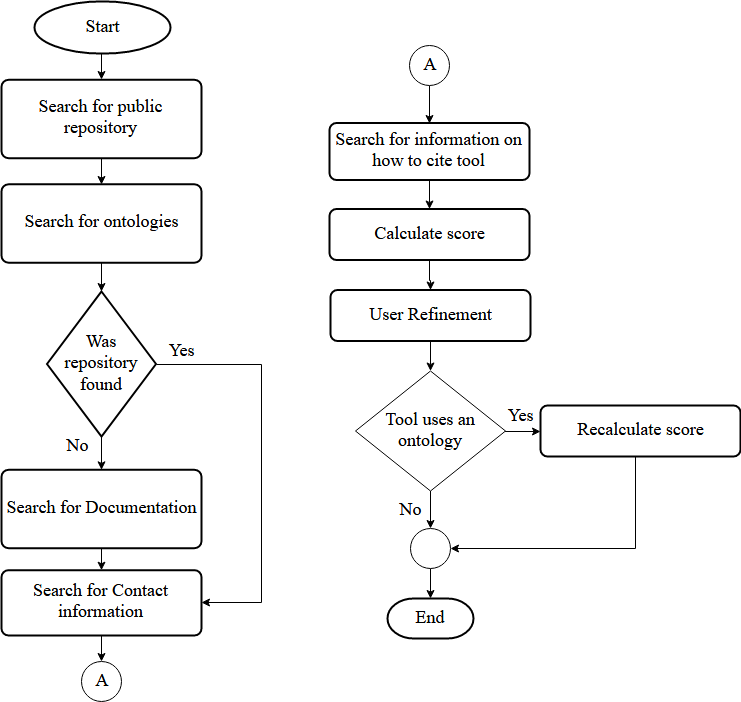
\includegraphics[width=\textwidth, height=\textheight, keepaspectratio]{Flowchart3.png}
	\caption{Flowchart showing calculation of Reusability.}
	\label{fig:flowchart3}
\end{figure}
\pagebreak
\subsection{Dataset FAIR Assessment}
This section will consider the computation involved in performing a FAIR assessment for a dataset. This starts by considering whether a dataset is findable on a website. If the website for the dataset is not found after filtering the links found from the Google Custom Search API, then the assessment will automatically fail, as there will be no way to gather information to automate the assessment.\newline
\textbf{Findability}\newline
The assessment tool then searches for information based on the second metric presented by this study for findability, that the dataset has a proper description. This is implemented by first searching for a link marked as ``About'', with the assumption that it would redirect you to a page providing information about the dataset. If no such link is found, the tool then searches for areas on the page named either as ``Introduction'', ``About'' or ``Description''. If no such area is found it then searches using XPath to see if an area in the HTML would be marked as ``desc''. If the information required is found, the description of the dataset is saved into the database and the points for this metric are awarded. This metric was given a medium priority. It carries 60\% of the dataset's total findability score.

The assessment tool then goes on to search for information based on the second metric presented in this study, i.e., dataset has a unique identifier. This is implemented by first searching the page for a link containing a DOI, which could be used as a direct link to the paper that presented that dataset. If a link is not found, the tool interfaces with Crossref using the Crossref API to search for the paper that presented the dataset by searching for the dataset's name.
\begin{lstlisting}[frame = single, caption={Searching Crossref API for paper presenting the dataset.}, captionpos=b]
w2 = works.query(title=dataset_name).filter
	(type=''journal-article").sort("relevance")
\end{lstlisting}
If a paper is found, the DOI is directly extracted from the paper and saved into the database, awarding points to the dataset for the metric. This metric was given a medium priority, equal to 40\% of the dataset's total findability score.
\begin{lstlisting}[frame = single, caption={Extracting DOI from paper.}, captionpos=b]
dataset_doi = item[`DOI']
\end{lstlisting}
\textbf{Accessibility}\newline
After calculating the dataset's findability, the assessment tool gathers information to calculate its accessibility. This process first begins by searching for information based on the first metric presented by this study, that the dataset is freely downloadable from the website. This is implemented by having the tool search the website for a link marked as ``Download''. If a link is found, it is assumed that it will take you to a download page where the dataset can be downloaded. This metric is given a high priority, equal to 80\% of the dataset's total accessibility score.

The second metric presented by the study is that metadata will still be available even if data is no longer available. This is covered by the previous process to search for the paper presenting this dataset. If a paper is found, it is automatically assumed that the metadata will be permanently available in that paper, awarding full points to the dataset for this metric. This metric carries 20\% of the total accessibility score as it is given a low priority.\newline
\textbf{Interoperability}\newline
The assessment tool then searches through the website for information to calculate the dataset's interoperability. This starts by considering the metric presented by this study to calculate the dataset's interoperability, information is provided on what format(s) or file format(s) the dataset is available in. This is implemented by searching the web page for areas containing the text ``file format'' or ``format''. If this area is found, it is assumed that this area provides the necessary information to fulfil this metric. This metric is given medium priority, however it is the sole metric that is used to calculate interoperability and carries 100\% of the interoperability score.\newline
\textbf{Reusability}\newline
Finally the assessment tool calculates the dataset's reusability. This starts by searching for information based on the first metric presented by this study, i.e., information is provided on how to cite the dataset. This is implemented by searching for an area in the web page by XPath containing the text ``Cite'', ``Citation'', ``Citing'' or ``References''. If this area is found, it is assumed that this area provides information on how to cite or reference the dataset. This metric is given a low priority and carries 33.3\% of the total reusability score. 

The assessment tool then searches for information based on the second metric presented by this study for reusability, that contact information is provided for the creator(s) of the dataset. This is implemented by first searching the web page for a link marked as ``Contact''. If the link is not found, then the assessment tool will search the page for an area by XPath containing the text ``email''. If an email link or area is found, then it is assumed that the email of the creator of the dataset is given. As such the criteria for this metric would be satisfied and the points for this metric would be awarded. This metric is given a low priority and carries 33.3\% of the total reusability score.

The assessment tool then goes on to search for information based on the final metric presented in this study for reusability, i.e., previous versions of the dataset are made available. This is implemented by searching through the web page for a link marked as ``Previous versions'' or ``Older versions''. If a link is found, it is assumed that previous versions of the dataset are available, fulfilling this metric. This metric carries 33.3\% of the dataset's total reusability score as it is given a low priority.\pagebreak
\subsection{Pipeline FAIR Assessment}
After calculating the FAIR score for the various tools and datasets, the user can then create a pipeline out of them. The pipeline itself can have a FAIR score which is calculated based on the FAIR score of the various tools and datasets in it.\newline\newline
Pipeline Findability:\newline
This is calculated by adding the findability of the various tools and datasets and dividing them by the total number of tools and datasets in the pipeline.\newline
\begin{equation}
\frac{Findability_{T1} + Findability_{D1} + ... + Findability_{Tn} + Findability_{Dn}}{N_{T}+N_{D}}
\end{equation}
\newline Pipeline Accessibility:\newline
This is calculated by adding the accessibility of the various tools and datasets and dividing them by the total number of tools and datasets in the pipeline.\newline
\begin{equation}
\frac{Accessibility_{T1} + Accessibility_{D1} + ... + Accessibility_{Tn} + Accessibility_{Dn}}{N_{T}+N_{D}}
\end{equation}
\newline Pipeline Interoperability:\newline
This is calculated by adding the interoperability of the various tools and datasets and dividing them by the total number of tools and datasets in the pipeline.\newline
\begin{equation}
\frac{Interoperability_{T1} + Interoperability_{D1} + ... + Interoperability_{Tn} + Interoperability_{Dn}}{N_{T}+N_{D}}
\end{equation}
\newline Pipeline Reusability:\newline
This is calculated by adding the reusability of the various tools and datasets and dividing them by the total number of tools and datasets in the pipeline.\newline
\begin{equation}
\frac{Reusability_{T1} + Reusability_{D1} + ... + Reusability_{Tn} + Reusability_{Dn}}{N_{T}+N_{D}}
\end{equation}
\section{Obtaining Data}
Along with the sets of tools and datasets required to test the system, some other sets of data were first gathered in order for the system to be implemented. The first set of data was the list of most commonly used phrases in bioinformatics. The data in this set was taken from the Bioinformatics glossary presented by Biosynthesis \cite{biogloss}. Not all the terms presented in this glossary were used. Instead, the list was created using the terms presented in the glossary which were most commonly used in websites of tools and datasets.

The second set of data that needed to be obtained was the list of active ontologies. This list would be used to be able to fulfil the metric presented for reusability of tools, i.e., the tool uses a community accepted ontology. In this case, the active tools would serve as community accepted ontologies. This list of ontologies was obtained from the OBO Foundry \cite{obo} in a YAML format. The following code was executed in order to obtain this list of ontologies.
\begin{lstlisting}[frame = single, caption={Obtaining list of ontologies from YAML file.}, captionpos=b, language=Python]
active_ontologies = []
with open("ontologies.yml", 'r') as ont:
  content = yaml.load(ont)
  for item in content.items():
      x = item[1]
      for i in range(len(x)):
          if x[i]["activity_status"] == "active":
              active_ontologies.append
              (x[i]["title"].lower())
\end{lstlisting}
The following is a list of some of the active ontologies used in this study:
\begin{multicols}{2}
\begin{itemize}
	\item Xenopus Anatomy Ontology; \item Zebrafish anatomy and development ontology; \item Human Disease Ontology;
	\item Gene Ontology; \item Basic Formal Ontology \item Evidence Ontology; \item Drug-drug Interactioon and drug Interaction Evidence Ontology;
	\item Human phenotype ontology.
\end{itemize}
\end{multicols}
A complete list of all the active ontologies used in this study can be found in Appendix A.
\chapter{Testing and Evaluation}
In this chapter, the testing of the system will be discussed, and the results obtained from the system will be evaluated. 

\section{Specification}
The system presented in this study is aimed at providing users with a way to obtain an assessment of a tool's findability, accessibility, interoperability and reusability. As such, the tests performed on this system are meant to achieve two main goals.

Firstly, the tests performed on the system are aimed to answer one of the research questions presented in the first chapter of this study: Can the FAIR assessment be part of an automated process? In order to be able to answer this question the tests were performed in the following manner. The assessment tool is first applied to a list of tools and datasets which were assessed by the FAIRshake tool assessment and the FAIRshake dataset assessment respectively. The results obtained were then compared with those found in the assessments made by FAIRshake to ensure that the automated assessment tool was able to find the information required to fulfil the metrics. The assessment tool will then be applied to a list of tools hosted by EMBL EBI \cite{ebi}, which will first have to be manually assessed. This manual assessment gives us a list of results that should be expected from the assessment tool, to ensure that it is working as expected. This is further assured through the use of Selenium (2018), which allows us to see which areas of a tool's website the tool is checking in order to obtain the required information.

The second goal of these tests is to ensure that the assessment provided by this study is justifiable and truly FAIR compliant. This is done by comparing the values of the results obtained from the automated assessment tool with the results presented by the FAIRshake tool and dataset assessments. A difference between the total scores of findability, accessibility, interoperability and reusability is expected due to the fact that different metrics are given different priorities in this study, whereas in the FAIRshake assessments, each metric is given the same priority. However, although this difference in totals is expected, this difference is not expected to be significant.

\section{Results}
In this section, the results from the tests performed on each set of tools and datasets will be discussed. Since the system presented in this study uses a priority system to distinguish the tools that are truly findable from those that fulfil only some minor criteria, the total result of each metric of findability, accessibility, interoperability and reusability will not be evaluated. The focus will instead be on the individual metrics, comparing how the tool compares to the results from the FAIRshake tool and dataset assessments \cite{FAIRshake} to see if the objective presented by this study holds (i.e. to automate as much of the FAIR assessment as possible). 
\subsection{FAIRshake Tools}
The evaluation considers the tools which were already assessed by the FAIRshake tool assessment \cite{FAIRshake} and compares the results obtained from the tool with the results from FAIRshake. It should be noted that the results given for Reusability have been refined to indicate whether a tool uses an ontology or not. This is to ensure that the provided FAIR score is not negatively affected by a metric that would otherwise not be applicable to the tool. 


\begin{table}[h]
\resizebox{\textwidth}{!}{%
{\renewcommand{\arraystretch}{1.5}%
\begin{tabular}{|c|l|c|c|c|c|l|c|c|c|c|}
\cline{1-1} \cline{3-6} \cline{8-11}
\textbf{} &  & \multicolumn{4}{c|}{\textbf{FAIRshake}} &  & \multicolumn{4}{c|}{\textbf{Automated Tool}} \\ \cline{3-6} \cline{8-11} 
\textbf{Tool} &  & \textbf{F} & \textbf{A} & \textbf{I} & \textbf{R} &  & \textbf{F} & \textbf{A} & \textbf{I} & \textbf{R} \\ \cline{1-1} \cline{3-6} \cline{8-11} 
BLAST &  & 75\% & 100\% & N/A & 75\% &  & 65\% & 100\% & 50\% & 50\% \\ \cline{1-1} \cline{3-6} \cline{8-11} 
HAMMOCK &  & 100\% & 100\% & N/A & 40\% &  & 75\% & 50\% & 50\% & 75\% \\ \cline{1-1} \cline{3-6} \cline{8-11} 
PyroHMMvar &  & 100\% & 0\% & N/A & 40\% &  & 75\% & 50\% & 50\% & 100\% \\ \cline{1-1} \cline{3-6} \cline{8-11} 
CytoSPADE &  & 75\% & 0\% & N/A & 20\% &  & 100\% & 0\% & 50\% & 75\% \\ \cline{1-1} \cline{3-6} \cline{8-11} 
MEANS &  & 100\% & 0\% & N/A & 60\% &  & 75\% & 50\% & 100\% & 75\% \\ \cline{1-1} \cline{3-6} \cline{8-11} 
poretools &  & 100\% & 0\% & N/A & 50\% &  & 75\% & 0\% & 100\% & 75\% \\ \cline{1-1} \cline{3-6} \cline{8-11} 
miRPathDB &  & 75\% & 0\% & N/A & 80\% &  & 65\% & 0\% & 0\% & 50\% \\ \cline{1-1} \cline{3-6} \cline{8-11} 
CHRONOS &  & 36\% & 100\% & N/A & 90\% &  & 90\% & 50\% & 83.33\% & 100\% \\ \cline{1-1} \cline{3-6} \cline{8-11} 
PhosphoPICK &  & 75\% & 0\% & N/A & 40\% &  & 90\% & 0\% & 0\% & 25\% \\ \cline{1-1} \cline{3-6} \cline{8-11} 
Breakpointer &  & 100\% & 0\% & N/A & 80\% &  & 75\% & 50\% & 66.67\% & 87.5\% \\ \cline{1-1} \cline{3-6} \cline{8-11} 
\end{tabular}%
}}
\caption{Comparison of results between FAIRshake assessment on tools and assessment made by the automated assessment tool.}
\label{tab:my-table}
\end{table}

\begin{table}[h]
{\renewcommand{\arraystretch}{1.5}%
\begin{tabular}{|c|l|c|c|c|c|}
\cline{1-1} \cline{3-6}
\textbf{} &  & \multicolumn{4}{c|}{Manual Assessment} \\
\textbf{Tool} &  & F & A & I & R \\ \cline{1-1} \cline{3-6} 
BLAST &  & 90\% & 100\% & 50\% & 50\% \\ \cline{1-1} \cline{3-6} 
HAMMOCK &  & 100\% & 100\% & 50\% & 75\% \\ \cline{1-1} \cline{3-6} 
PyroHMMvar &  & 100\% & 100\% & 50\% & 100\% \\ \cline{1-1} \cline{3-6} 
CytoSPADE &  & 100\% & 0\% & 50\% & 75\% \\ \cline{1-1} \cline{3-6} 
MEANS &  & 100\% & 100\% & 100\% & 75\% \\ \cline{1-1} \cline{3-6} 
poretools &  & 100\% & 50\% & 100\% & 75\% \\ \cline{1-1} \cline{3-6} 
miRPathDB &  & 90\% & 50\% & 0\% & 50\% \\ \cline{1-1} \cline{3-6} 
CHRONOS &  & 90\% & 50\% & 83.33\% & 100\% \\ \cline{1-1} \cline{3-6} 
PhosphoPICK &  & 90\% & 0\% & 0\% & 25\% \\ \cline{1-1} \cline{3-6} 
Breakpointer &  & 100\% & 50\% & 66.67\% & 87.5\% \\ \cline{1-1} \cline{3-6} 
\end{tabular}
}
\caption{Manual assessment on tools from FAIRshake tool assessment.}
\label{tab:my-table}
\end{table}

The evaluation considers the total scores of findability, accessibility, interoperability and reusability of the FAIRshake assessment and the results obtained from the automated assessment tool. This is done to ensure that although metrics are given different priorities, there is not a significant difference between the score obtained by the assessment tool and those given by FAIRshake. By checking which scores have significant differences and checking the results obtained in the metrics presented by that principle, it is possible to check where differences in the results rose from.
\begin{itemize}
	\item Findability:
		\begin{itemize}
			\item The main reason for the differences in findability scores was that the automated assessment tool was unable to find a DOI linking to the paper that presented the tool, as can be seen in the table 5.1 for BLAST, HAMMOCK, PyroHMMvar, CytoSPADE, MEANS, poretools, miRPathDB and Breakpointer. This resulted in lower scores, but when the information is provided, the score is more accurate and richer.
		\end{itemize}
	\item Accessibility:
		\begin{itemize}
			\item The main reason for a difference in accessibility scores was the fact that another metric was presented in this study, which is not provided by FAIRshake, as can be seen in table 5.1 for HAMMOCK, PyroHMMvar, CHRONOS and Breakpointer. This resulted in lower scores when the automated tool found the same information as FAIRshake but did not find information to satisfy the metrics presented in this study as can be seen for HAMMOCK and CHRONOS. On the other hand, this resulted in a higher score when the FAIRshake metric was not satisfied but the automated tool found information to satisfy the metric presented by this study as can be seen for PyroHMMvar and Breakpointer.
		\end{itemize}
	\item Reusability:
		\begin{itemize}
			\item One of the reasons for a difference in reusability scores was the fact that this study uses different priorities for its metrics, so although it was able to find the same information as FAIRshake, the final result was different. Another reason why there was a difference was that for HAMMOCK, PyroHMMvar and CytoSPADE, a public repository was added after the assessment was performed by FAIRshake. Furthermore, although the difference may seem very large, this can be explained by the fact that the first metric of a tool's Reusability, i.e., the tool is hosted in a public repository, was given a high priority. This metric carries 50\% of the total reusability score, which is the reason for a seemingly large difference in scores in the case of BLAST, miRPathDB and PhosphoPICK, as can be seen in table 5.1.
		\end{itemize}
\end{itemize}
\subsection{EMBL EBI Tools}
Moving on to the tools hosted by the EMBL EBI \cite{ebi}, the evaluation can now compare the results obtained from a manual assessment with those obtained from the automated assessment tool. The manual assessment was performed using all the metrics presented by this study, including the metrics for accessibility and interoperability that were not provided by FAIRshake and providing a score based on their priority. Similar to the previous set of tools, the results given for reusability have been adjusted to indicate whether a tool uses an ontology or not.

\begin{table}[h]
\resizebox{\textwidth}{!}{%
{\renewcommand{\arraystretch}{1.5}%
\begin{tabular}{|c|l|c|c|c|c|l|c|c|c|c|}
\cline{1-1} \cline{3-6} \cline{8-11}
\textbf{} &  & \multicolumn{4}{c|}{\textbf{Manual Assessment}} &  & \multicolumn{4}{c|}{\textbf{Automated Tool}} \\ \cline{3-6} \cline{8-11} 
\textbf{Tool} &  & \textbf{F} & \textbf{A} & \textbf{I} & \textbf{R} &  & \textbf{F} & \textbf{A} & \textbf{I} & \textbf{R} \\ \cline{1-1} \cline{3-6} \cline{8-11} 
Clustal Omega &  & 90\% & 100\% & 100\% & 100\% &  & 65\% & 100\% & 100\% & 100\% \\ \cline{1-1} \cline{3-6} \cline{8-11} 
HMMER &  & 100\% & 50\% & 50\% & 87.5\% &  & 75\% & 50\% & 50\% & 87.5\% \\ \cline{1-1} \cline{3-6} \cline{8-11} 
FASTA &  & 100\% & 50\% & 100\% & 100\% &  & 75\% & 50\% & 100\% & 100\% \\ \cline{1-1} \cline{3-6} \cline{8-11} 
Phobius &  & 90\% & 0\% & 0\% & 50\% &  & 90\% & 0\% & 0\% & 50\% \\ \cline{1-1} \cline{3-6} \cline{8-11} 
InterProScan &  & 100\% & 50\% & 66.67\% & 87.5\% &  & 75\% & 50\% & 66.67\% & 87.5\% \\ \cline{1-1} \cline{3-6} \cline{8-11} 
\end{tabular}%
}}
\caption{Comparison of results between a manual assessment performed on EMBL EBI tools and assessment performed by the automated assessment tool.}
\label{tab:my-table}
\end{table}

By comparing the results obtained, we can see whether the automated assessment tool is working as expected. In cases of differences we can see that differences can be observed in findability scores. All of these occurrences were due to the fact that the automated assessment tool was unable to find a DOI linking to the paper that presented the tool, as can be seen in table 5.2 for Clustal Omega, HMMER, FASTA and InterProScan. The paper presenting the tools were found through extensive searches through literature in order to find the papers that presented the tools. After the assessment is performed and a score is provided, the user will be able to refine the score and provide any missing information.

\subsection{FAIRshake Datasets}
We can then see and compare the results from assessments made on datasets by FAIRshake and compare them with the results obtained from the automated assessment tool.

\begin{table}[h]
\resizebox{\textwidth}{!}{%
{\renewcommand{\arraystretch}{1.5}%
\begin{tabular}{|c|c|c|c|c|c|c|c|c|c|c|}
\cline{1-1} \cline{3-6} \cline{8-11}
\textbf{} &  & \multicolumn{4}{c|}{\textbf{FAIRshake}} &  & \multicolumn{4}{c|}{\textbf{Automated Tool}} \\ \cline{3-6} \cline{8-11} 
\textbf{Dataset} &  & \textbf{F} & \textbf{A} & \textbf{I} & \textbf{R} &  & \textbf{F} & \textbf{A} & \textbf{I} & \textbf{R} \\ \cline{1-1} \cline{3-6} \cline{8-11} 
\begin{tabular}[c]{@{}c@{}}A443654\\   KINOMEscan\end{tabular} &  & 50\% & 50\% & 100\% & 67\% &  & 60\% & 80\% & 100\% & 66.67\% \\ \cline{1-1} \cline{3-6} \cline{8-11} 
\begin{tabular}[c]{@{}c@{}}(R)-Roscovitine\\   KINOMEscan\end{tabular} &  & 50\% & 50\% & 100\% & 67\% &  & 60\% & 80\% & 100\% & 66.67\% \\ \cline{1-1} \cline{3-6} \cline{8-11} 
\begin{tabular}[c]{@{}c@{}}GTEx\\   Portal Datasets\end{tabular} &  & 50\% & 50\% & 100\% & 100\% &  & 60\% & 80\% & 100\% & 100\% \\ \cline{1-1} \cline{3-6} \cline{8-11} 
WormBase Datasets &  & 100\% & 100\% & 100\% & 100\% &  & 100\% & 100\% & 100\% & 100\% \\ \cline{1-1} \cline{3-6} \cline{8-11} 
\begin{tabular}[c]{@{}c@{}}Gene Ontology\\ Consortium Datasets\end{tabular} &  & 50\% & 50\% & 100\% & 67\% &  & 60\% & 80\% & 100\% & 66.67\% \\ \cline{1-1} \cline{3-6} \cline{8-11} 
\begin{tabular}[c]{@{}c@{}}Rat Genome \\ Database Datasets\end{tabular} &  & 50\% & 50\% & 100\% & 67\% &  & 60\% & 80\% & 100\% & 66.67\% \\ \cline{1-1} \cline{3-6} \cline{8-11} 
\end{tabular}%
}}
\caption{Comparison of results between FAIRshake assessment on datasets and assessment performed by the automated assessment tool.}
\label{tab:my-table}
\end{table}

The differences that can be observed in these results arise from the fact that the assessment tool gives different priorities to different metrics. However, all the information obtained by the automated tool for assessment is the same as that for FAIRshake.

\subsection{EMBL EBI Datasets}
Moving on to the datasets hosted by EMBL EBI \cite{ebi}. The following table compares the results obtained through a manual assessment with those obtained from the automated assessment tool. The manual assessment was performed using the metrics presented by this study and providing a score based on their priority.

\begin{table}[h!]
\resizebox{\textwidth}{!}{%
{\renewcommand{\arraystretch}{1.5}%
\begin{tabular}{|c|c|c|c|c|c|c|c|c|c|c|}
\cline{1-1} \cline{3-6} \cline{8-11}
\textbf{} &  & \multicolumn{4}{c|}{\textbf{Manual Assessment}} &  & \multicolumn{4}{c|}{\textbf{Automated Tool}} \\ \cline{3-6} \cline{8-11} 
\textbf{Dataset} &  & \textbf{F} & \textbf{A} & \textbf{I} & \textbf{R} &  & \textbf{F} & \textbf{A} & \textbf{I} & \textbf{R} \\ \cline{1-1} \cline{3-6} \cline{8-11} 
ArrayExpress &  & 100\% & 100\% & 100\% & 100\% &  & 100\% & 100\% & 100\% & 100\% \\ \cline{1-1} \cline{3-6} \cline{8-11} 
BioModels &  & 60\% & 80\% & 100\% & 66.67\% &  & 60\% & 80\% & 100\% & 66.67\% \\ \cline{1-1} \cline{3-6} \cline{8-11} 
InterPro &  & 100\% & 100\% & 100\% & 100\% &  & 100\% & 100\% & 100\% & 100\% \\ \cline{1-1} \cline{3-6} \cline{8-11} 
Pfam &  & 100\% & 100\% & 100\% & 100\% &  & 100\% & 100\% & 100\% & 100\% \\ \cline{1-1} \cline{3-6} \cline{8-11} 
\end{tabular}%
}}
\caption{Comparison of results between manual assessment performed on EMBL EBI datasets and assessment performed by the automated assessment tool.}
\label{tab:my-table}
\end{table}
The results show that the tool managed to obtain all the data necessary for an assessment as would be expected in a real-world scenario.

\subsection{Pipeline Tools}
Finally, we can compare the results obtained from manually assessing the tools in the pipeline presented by Barber et al. (2012) with the results obtained from the automated assessment tool. The manual assessment was performed using the metrics presented by this study and providing scores based on their priority.

\begin{table}[h]
\resizebox{\textwidth}{!}{%
{\renewcommand{\arraystretch}{1.5}%
\begin{tabular}{|c|c|c|c|c|c|c|c|c|c|c|}
\cline{1-1} \cline{3-6} \cline{8-11}
\textbf{} &  & \multicolumn{4}{c|}{\textbf{Manual Assessment}} &  & \multicolumn{4}{c|}{\textbf{Automated Tool}} \\ \cline{3-6} \cline{8-11} 
\textbf{Tool} &  & \textbf{F} & \textbf{A} & \textbf{I} & \textbf{R} &  & \textbf{F} & \textbf{A} & \textbf{I} & \textbf{R} \\ \cline{1-1} \cline{3-6} \cline{8-11} 
MUSCLE &  & 100\% & 50\% & 100\% & 100\% &  & 100\% & 50\% & 100\% & 100\% \\ \cline{1-1} \cline{3-6} \cline{8-11} 
Sequencher &  & 65\% & 100\% & 33.33\% & 12.5\% &  & 65\% & 100\% & 33.33\% & 12.5\% \\ \cline{1-1} \cline{3-6} \cline{8-11} 
MAFFT &  & 90\% & 50\% & 100\% & 75\% &  & 90\% & 50\% & 100\% & 75\% \\ \cline{1-1} \cline{3-6} \cline{8-11} 
jModelTest &  & 100\% & 50\% & 100\% & 100\% &  & 100\% & 50\% & 100\% & 100\% \\ \cline{1-1} \cline{3-6} \cline{8-11} 
RAxML &  & 100\% & 50\% & 100\% & 100\% &  & 100\% & 50\% & 100\% & 100\% \\ \cline{1-1} \cline{3-6} \cline{8-11} 
MrBayes &  & 100\% & 50\% & 100\% & 87.5\% &  & 75\% & 50\% & 100\% & 87.5\% \\ \cline{1-1} \cline{3-6} \cline{8-11} 
BEAST &  & 100\% & 100\% & 100\% & 100\% &  & 100\% & 100\% & 100\% & 100\% \\ \cline{1-1} \cline{3-6} \cline{8-11} 
DnaSP &  & 90\% & 100\% & 66.67\% & 37.5\% &  & 90\% & 100\% & 66.67\% & 37.5\% \\ \cline{1-1} \cline{3-6} \cline{8-11} 
\end{tabular}%
}}
\caption{Comparison of results between manual assessment performed on tools in pipeline presented by Barber et al. (2012) and assessment performed by the automated assessment tool.}
\label{tab:my-table}
\end{table}

A difference in Findability can be observed in table 5.5 for MrBayes, as the automated assessment tool was unable to find a DOI linking to the paper that presented the tool. The total findability, accessibility, interoperability and reusability of the pipeline were then calculated by the system. 


\begin{table}[h]
{\renewcommand{\arraystretch}{1.5}%
\begin{tabular}{|c|c|c|}
\hline
 & \textbf{Expected} & \textbf{Actual} \\ \hline
\textbf{Findability} & 93.12\% & 90\% \\ \hline
\textbf{Accessibility} & 68.75\% & 68.75\% \\ \hline
\textbf{Interoperability} & 87.5\% & 87.5\% \\ \hline
\textbf{Reusability} & 76.56\% & 76.56\% \\ \hline
\end{tabular}%
}
\caption{Comparison of pipeline expected FAIR score against actual FAIR score calculated by system.}
\label{tab:my-table}
\end{table}

The difference in Findability observed in table 5.5 for MrBayes affected the total Findability of the pipeline, resulting in a 3.12\% loss in findability. \pagebreak

\section{Evaluation of Results}
In this section, the results obtained will be further evaluated, by taking into consideration the two main goals which these tests aimed to achieve.

\subsection{Justifiable FAIR Score}
The first consideration is given to the secondary goal of these tests, i.e., are the metrics used for this study justifiable and truly FAIR?

In order to ensure that the metrics used in this study and the priority system used are truly FAIR, we must compare the total result obtained from the automated assessment tool with that provided by FAIRshake. Taking a look at table 5.1, we can see that although there are some differences in the results, even though both results have the same amount of passing metrics, the difference is not too large. For example, in the case of miRPathDB, both results have passed the same amount of metrics, however the metric that failed is given more priority in this study. This difference in priority has not led to a significant difference between the results.

Furthermore, this goal is further achieved through the additional metrics provided in order to ensure a more accurate FAIR score. As can be seen in table 5.1, some of the accessibility scores are very different. This is due to the fact that FAIRshake provides only one metric to calculate a tool's accessibility. In this study, a second metric was provided, in order to allow for a more refined and a more accurate FAIR score. This is also shown in the introduction of two metrics for the Interoperability of tools. This provides a more accurate and refined FAIR score over that of FAIRshake, which do not consider the Interoperability of tools altogether.

A similar observation can be made when looking at the results obtained by the automated assessment tool in the case of datasets. The results of the assessment tool are not too different from those presented by the FAIRshake data assessment, even though the metrics are given a different priority. In the case of datasets however, there are still very few metrics implemented to calculate their FAIR score.

\subsection{Answering the Hypothesis}
The main goal of the tests run on this system was to try and answer one of the research questions presented in this study, i.e., can the FAIR assessment be automated? 

Taking into consideration the first set of tools which the assessment was performed on, a few differences can be noted in some of the results. As can be seen in table 5.1, quite a few results were different. However some difference was expected due to the fact that the assessment tool presented in this study uses a different priority system. This is the case for the majority of the differences in accessibility and reusability. In the cases for accessibility, there are two metrics presented by this study, which results in a lower FAIR score if only the metric presented by FAIRshake applies. Furthermore, the difference in priorities for metrics presented by reusability account for the difference in almost all the tools, with the exception of HAMMOCK, PyroHMMvar and CytoSPADE, where a public repository was added after the assessment was performed by FAIRshake. On the other hand, a difference can be noted in the Findability of a majority of the tools as shown in table 5.1. Further inspection showed that the differences all rose from the same metric, i.e., the tool has a unique identifier. This can be seen for BLAST and MEANS in table 5.8 below.

\begin{table}[h]
\resizebox{\textwidth}{!}{%
{\renewcommand{\arraystretch}{1.5}%
\begin{tabular}{|c|l|c|c|}
\cline{1-1} \cline{3-4}
\textbf{BLAST} &  & \textbf{FAIRshake assessment} & \textbf{Automated Assessment} \\ \cline{1-1} \cline{3-4} 
\textbf{Findability} &  & \textbf{75\%} & \textbf{65\%} \\ \cline{1-1} \cline{3-4} 
Tool is freely downloadable. &  & 25\% & 40\% \\ \cline{1-1} \cline{3-4} 
Tool has a proper description. &  & 25\% & 25\% \\ \cline{1-1} \cline{3-4} 
\begin{tabular}[c]{@{}c@{}}Previous versions of tool\\ are available.\end{tabular} &  & 0\% & 0\% \\ \cline{1-1} \cline{3-4} 
Tool has a unique identifier. &  & 25\% & 0\% \\ \cline{1-1} \cline{3-4} 
\textbf{MEANS} & \multicolumn{1}{c|}{} &  &  \\ \cline{1-1} \cline{3-4} 
\textbf{Findability} & \multicolumn{1}{c|}{} & \textbf{100\%} & \textbf{75\%} \\ \cline{1-1} \cline{3-4} 
Tool is freely downloadable. & \multicolumn{1}{c|}{} & 25\% & 40\% \\ \cline{1-1} \cline{3-4} 
Tool has a proper description. & \multicolumn{1}{c|}{} & 25\% & 25\% \\ \cline{1-1} \cline{3-4} 
\begin{tabular}[c]{@{}c@{}}Previous versions of tool\\ are available.\end{tabular} & \multicolumn{1}{c|}{} & 25\% & 10\% \\ \cline{1-1} \cline{3-4} 
Tool has a unique identifier. & \multicolumn{1}{c|}{} & 25\% & 0\% \\ \cline{1-1} \cline{3-4} 
\end{tabular}%
}}
\caption{Comparison of Findability metrics for BLAST and MEANS.}
\label{tab:my-table}
\end{table}

A set of tests were then performed on tools hosted by EMBL EBI \cite{ebi}. These tests were performed using all the metrics provided by this study, taking into consideration the developed priority system as well as the metrics which were not considered by FAIRshake. As can be seen in table 5.2, due to these considerations the differences that were found in accessibility, interoperability and reusability were no longer present. This further shows that the differences that arose in these areas were all from the different weightings given in the system presented by this study. The differences in the scores of findability, however, were still present. Further inspection of the results showed that almost every tool, with the exception of Phobius, failed the same metric as the first set of tools, i.e, the tool has a unique identifier.


From the manual assessment of tools, some difficulty was found in locating the papers that presented the tools. This was because the websites do not follow a ``pattern'' that would allow for easily findable information. Some of the required information was scattered around the web page, which made it very difficult to find. This was then further shown through the automated assessment tool in its inability to find the required unique identifier for the majority of the tools. 

On the other hand, the results obtained for datasets contain very few differences. As can be seen in table 5.3, most of the differences between the total results are small, all of which could be attributed to the fact that the system presented in this study uses a different priority system than that of FAIRshake. A comparison of metrics for A443654KINOMEscan is shown in table 5.9 below. The results of the second set of datasets on which the automated assessment tool was applied further indicate this trend. The results obtained from the manual assessment and the automated assessment tool were the same, which means that for the metrics presented for datasets, the FAIR assessment can be sufficiently automated.

\begin{table}[h]
\resizebox{\textwidth}{!}{%
{\renewcommand{\arraystretch}{1.5}%
\begin{tabular}{|c|c|c|c|}
\cline{1-1} \cline{3-4}
\textbf{A443654KINOMEscan} & \multicolumn{1}{l|}{} & \textbf{FAIRshake assessment} & \textbf{Automated Assessment} \\ \cline{1-1} \cline{3-4} 
\textbf{Findability} & \multicolumn{1}{l|}{} & \textbf{50\%} & \textbf{60\%} \\ \cline{1-1} \cline{3-4} 
\begin{tabular}[c]{@{}c@{}}Information about dataset is\\ provided.\end{tabular} & \multicolumn{1}{l|}{} & 100\% & 60\% \\ \cline{1-1} \cline{3-4} 
Dataset has a unique identifier. & \multicolumn{1}{l|}{} & 0\% & 0\% \\ \cline{1-1} \cline{3-4} 
\textbf{Accessibility} & \multicolumn{1}{l|}{} & \textbf{50\%} & \textbf{80\%} \\ \cline{1-1} \cline{3-4} 
Dataset is freely downloadable. & \multicolumn{1}{l|}{} & 50\% & 80\% \\ \cline{1-1} \cline{3-4} 
\begin{tabular}[c]{@{}c@{}}Information about dataset will\\ persist after dataset becomes\\ unavailable.\end{tabular} &  & 0\% & 0\% \\ \cline{1-1} \cline{3-4} 
\textbf{Interoperability} &  & \textbf{100\%} & \textbf{100\%} \\ \cline{1-1} \cline{3-4} 
\begin{tabular}[c]{@{}c@{}}Information is given on which\\ file formats the dataset\\ is available in.\end{tabular} &  & 100\% & 100\% \\ \cline{1-1} \cline{3-4} 
\textbf{Reusability} &  & \textbf{67\%} & \textbf{66.67\%} \\ \cline{1-1} \cline{3-4} 
\begin{tabular}[c]{@{}c@{}}Information on how to cite \\ dataset is provided.\end{tabular} &  & 33\% & 33.33\% \\ \cline{1-1} \cline{3-4} 
\begin{tabular}[c]{@{}c@{}}Dataset developer's contact\\ information is provided.\end{tabular} &  & 0\% & 0\% \\ \cline{1-1} \cline{3-4} 
\begin{tabular}[c]{@{}c@{}}Previous versions of\\ dataset are available.\end{tabular} &  & 34\% & 33.33\% \\ \cline{1-1} \cline{3-4} 
\end{tabular}%
}}
\caption{Comparison of FAIR metrics for A443654KINOMEscan.}
\label{tab:my-table}
\end{table}

Finally, the results for the set of tools in the pipelines show that the same issue in the first two sets of tools is also present in this context. This issue of not being able to find a DOI linking to the paper that presented the tool, however, is not as apparent as in the other two sets, as it only affected one of the tools in this set, i.e., MrBayes. Similar to the tools in the other sets, it was very difficult to find the DOI of the paper presenting this tool, which in turn resulted in the automated assessment tool being unable to find it. In this scenario, it did not have a large effect on the pipeline's total findability score, as it was only 3.12\% lower than the expected score. However, the majority of the tools which were tested suffered from this issue. If a pipeline in bioinformatics follows the same pattern, then the system will provide a poor findability score, even though a unique identifier exists. The DOI can be given manually by a user at a later stage.

In conclusion, in the case of the datasets, the tests proved that the information required is quite easily findable, resulting in a proper FAIR score as expected. Therefore in the case of datasets, the hypothesis of whether or not the assessment can be automated passes. In the case of tools, however, the assessment might not be fully automate-able. Firstly, the second metric presented for reusability, i.e., the tool uses a community accepted ontology, cannot be automated at all, as there is no way to tell when a tool doesn't use ontologies altogether. In  such cases, it is up to the user to refine the result to provide a more accurate FAIR score. Furthermore, a common problem was found in calculating the findability for tools in that the unique identifier is not always made findable. In these cases, the findability score would be lower than it should be simply because the information is not findable by automated means.
\chapter{Future Work}
Future works in this study concern further improvements being made to the assessment metrics, specifically those for tool accessibility and dataset metrics. In its current state, there are very few metrics that relate to a dataset's findability, accessibility, interoperability and reusability, and very little research available on what metrics can be used in order to calculate such a score. An improvement can be made by increasing these metrics in order to obtain a more accurate FAIR score.\newline

Furthermore, in its current state, the system is slow at calculating a tool's or dataset's FAIR score. In the case where a large pipeline needs to be assessed, it can take quite some time to calculate the FAIR score of each individual tool and dataset. As such, an improvement can be made by implementing multi-threading techniques in the assessment in order to speed up the process.\newline

Another improvement that can be made that would improve the system's efficiency would be to use a different technology for web crawling. For the purpose of this study, Selenium (2018) was used as it allowed us to better visualize the web scraping process. However, this slows down the FAIR assessment quite significantly. Using a different system to for web crawling will therefore improve the speed at which information is obtained from the web pages, leading to the faster calculation of a tool or dataset's FAIR score.

\chapter{Conclusions}
Data in the biological field will still continue to be generated at a very fast rate, along with tools that will aid in the processing of this data. It is important to ensure that the data being generated is reproducible, to allow researchers to reproduce the results obtained to strengthen their own findings \cite{nature} This increase in data will continue to make it difficult for researchers to find the resources they need for their research which will slow down scientific progress. Studies have presented guidelines and metrics in order to evaluate a tool's Findability, Accessibility, Interoperability and Reusability in order to help users find the appropriate resource  for their task. 

This study aims to provide researchers with a searchable archive of tools and datasets, as well as provide a means to automate the calculation of FAIR scores for these resources. These aims were achieved through the use of web crawling techniques which were used to obtain the information required to calculate a FAIR score in an automated way. Furthermore, the use of web frameworks and database management systems allowed us to create a portal which acts as a front-end to the user, allowing them to search for the required resource by its features or capability and see the respective FAIR scores. This will allow the user to see what areas in Findability, Accessibility, Interoperability or Reusability the tool is lacking in, and what is required in order to improve that resource's FAIR score.

Sets of tools and datasets obtained from different sources were used to test the system. A set of tools and datasets obtained from the FAIRshake tool and dataset assessments were used to ensure that the FAIR assessment can be automated, by comparing the results obtained from the tool with those obtained from FAIRshake. The automation of the assessment was further shown through manual assessments of a set of tools and datasets obtained from EMBL EBI \cite{ebi} and comparing the results from the manual assessments with those obtained from the automated tool. 

The evaluation provided further insight and answers to the proposed specifications. By comparing the results of the individual metrics from the tools and datasets obtained from FAIRshake with those obtained from the system presented by this study, it can be observed that the system was able to obtain the information necessary in order to fulfil the metrics presented and provide a proper FAIR score. These observations were then further proven through the manual assessments of the tools and datasets obtained from EMBL EBI \cite{ebi} and the tools used in the pipeline presented by Barber et al. (2012). The manual assessments were performed using the metrics presented in this study, taking into considerations the additional metrics that were not considered by FAIRshake, as well as the different priority system used in this study. The results obtained show that the tool was able to obtain the same results as those obtained by the manual assessments, proving that the tool performs as expected, with a few exceptions in the case of tools where the tool struggled to find a tool's unique identifier.

It can be concluded that the aims and objectives presented by this study have been achieved. The results of the individual metrics obtained from testing are consistent with those obtained from FAIRshake, showing that it is possible for the FAIR assessment to be part of an automated process. The portal then allows users to search for their required tool and provides them with a FAIR score that can aid them to decide on which tool they should choose.


\begin{appendices}
\chapter{List of Active Ontologies}
\begin{multicols}{2}
\begin{itemize}
	\item Plant Ontology; \item Xenopus Anatomy Ontology; \item Zebrafish anatomy and development ontology;
	\item Ontology for Biomedical Investigations; \item Gene Ontology; \item Basic Formal Ontology;
	\item Phenotype And Trait Ontology; \item Human Disease Ontology; \item Chemical Entities of Biological Interest;
	\item PRotein Ontology (PRO); \item Ontology of Vaccine Adverse Events; \item Fungal gross anatomy;
	\item Gazetter; \item Ontology for MIRNA Target; \item Hymenoptera Anatomy Ontology;
	\item Information Artifact Ontology; \item Rat Strain Ontology; \item Foundational Model of Anatomy Ontology (subset)
	\item RNA ontology; \item eagle-i resource ontology; \item Genotype Ontology;
	\item Evidence ontology; \item Social Insect Behaviour Ontology; \item Ontology of Biological and Clinical Statistics;
	\item Tick Anatomy Ontology; \item Ontology for General Medical Science; \item Agronomy Ontology;
	\item Drug-drug Interaction and drug Interaction Evidence Ontology; \item Cardiovascular Disease Ontology;
	\item Biological Imaging Methods Ontology; \item Mouse pathology ontology; \item Pathogen Transmission Ontology; \item Cell Ontology;
	\item Unified phenotype ontology (uPheno); \item Xenopus Phenotype Ontology; \item Kinetic Simulation Algorithm Ontology; \item Mammalian Phenotype
	\item Experimental condition ontology; \item Exposure ontology; \item Geographical Entity Ontology; \item Units of measurement ontology; \item FOODON; \item Pathway ontology;
	\item Homology Ontology; \item Mammalian Feeding Muscle Ontology; \item Spider Ontology; \item Medaka Developmental Stages; \item FlyBase Controlled Vocabulary; \item Planarian Phenotype Ontology; \item Software ontology; \item Informed Consent Ontology;
	\item Drosophila gross anatomy; \item Common Anatomy Reference Ontology; \item Systems Biology Ontology; \item Platynereis Developmental Stages; \item Ontology of Genetic Susceptibility Factor; \item Ontology of core ecological entities; 
	\item Ontology of Biological Attributes; \item Beta Cell Genomics Ontology; \item MHC Restriction Ontology; \item Ontology of Medically Related Social Entities; \item Genomic Epidemiology Ontology;
	\item The Prescription of Drugs Ontology; \item Ontology for Biobanking; \item The Oral Health and Disease Ontology; \item Drosophila Phenotype Ontology; \item Clinical measurement ontology; \item human phenotype ontology;
	\item Pathogen Host Interaction Phenotype Ontology; \item Sequence types and features ontology; Ontology of Microbial Phenotypes; \item Mental Disease Ontology; \item Ontology of Precision Medicine and Investigation;
	\item EuPathDB ontology; \item NCBI organismal classification; \item Mouse adult gross anatomy; \item The Data Use Ontology; \item C. elegans Gross Anatomy Ontology; \item Protein Modification; \item Flora Phenotype Ontology; \item Relation Ontology;
	\item Dictyostelium discoideum anatomy; \item Minimum PDDI Information Ontology; \item Mass spectrometry ontology; \item Confidence Information Ontology; \item Non-Coding RNA Ontology; \item Ontology of Adverse Events;
	\item Emotion Ontology; \item The Statistical Methods Ontology; \item The Drug Ontology; \item Vertebrate trait ontology; \item Mathematical modelling ontology; \item Molecular Interactions Controlled Vocabulary; \item Biological Collections Ontology; \item MIAPA Ontology;
	\item Mental Functioning Ontology; \item Zebrafish developmental stages ontology; \item Microbial Conditions Ontology; \item Anatomical Entity Ontology; \item Infectious Disease Ontology; \item Mouse gross anatomy and development, timed; \item Vertebrate Taxonomy Ontology;
	\item Ontology for Parasite LifeCycle; \item Ontology of Host-Microbiome Interactions; \item Mouse Developmental Stages; \item Fission Yeast Phenotype Ontology; \item Zebrafish Phenotype Ontology; \item The Drug-Drug Interactions Ontology; \item Comparative Data Analysis Ontology;
	\item Human Developmental Stages; \item Biological Spatial Ontology; \item Plant Experimental Conditions Ontology; \item Ontology of Arthropod Circulatory Systems; \item Vaccine Ontology; \item Monarch Disease Ontology; \item Asocmycete phenotype ontology; \item Contributor Role Ontology; 
	\item microRNA Ontology; \item Chemical Information Ontology; \item Plant Phenology Ontology; \item Chemical Methods Ontology; \item Drosophila development; \item Ontology of Prokaryotic Phenotypic and Metabolic Characters; \item Name Reaction Ontology; \item Interaction Network Ontology; 
	\item Ontologized MIABIS; \item Obstetric and Neonatal Ontology; \item Symptom Ontology; \item Mosquito insecticide resistance; \item C. elegans phenotype; \item Uberon multi-species anatomy ontology; \item Measurement method ontology; \item Taxonomic rank vocabulary; \item Cell Line Ontology; \item Ctenophore Ontology;
	\item Teleost taxanomy ontology; \item Neuro Behaviour Ontology; \item Malaria Ontology; \item NCI Thesaurus OBO Edition; \item Porifera Ontology; \item Antibiotic Resistance Ontolgoy; \item Environment Ontology; \item planaria-ontology; \item Plant Trait Ontology; \item Dictyostelium discoideum phenotype ontology;
	\item Population and Community ontology; \item Molecular Process Ontology; \item Zebrafish Experimental Conditions Ontology; \item Scientific Evidence and Provenace Information Ontology; \item The Ontolgoy of Genes and Genomes; \item Human Ancestry Ontolgoy; \item Mosquito grass anatomy ontology; 
	\item BRENDA tissue/enzyme source.
\end{itemize}
\end{multicols}
\end{appendices}
\nocite{*}
\bibliography{refs}
\bibliographystyle{apacite}

\end{document}